\chapter{Transcriptional differences between WT and TG mice}\label{ch: transcriptional_global_differences}
%Classification of AS events, which most commonly observed/dominant? Isoforms derived from transcriptional regulation (alternative promoters) vs post-transcriptional regulation? 
%Impact of AS events on protein domains. Non-sense mediated decay? 
%%Furthermore changes in gene/transcript expression can be due to differences in cellular composition (i.e. neuronal loss/reactive gliosis) rather than indicative of disease-associated transcriptional regulation. 
%%Gene expression and mRNA isoforms vary widely across tissues (\cite{Wang2008}), thus sequencing the disease-relevant tissue (in this case entorhinal cortex) is important for understanding the pathology of AD. However, it is consequently important to note that other tissues may have to be considered to fully grasp the whole picture of AD development. 

\section{Introduction}

Following the accurate characterisation of the mouse transcriptome using long-read sequencing from a global (whole transcriptome approach, \cref{ch: whole_transcriptome}), this chapter aims to exploit these datasets to investigate the transcriptional changes in the mouse entorhinal cortex associated with tau pathology. 

There have been multiple studies recently that explore the transcriptional differences in transgenic mice harbouring different mutations associated with AD. However, all of these studies to date have been undertaken with short-read RNA-Seq - which, while it offers obvious advantage compared to microarrays in accurately quantifying gene expression, is severely limited in detecting and characterising transcripts (as discussed in detail in \cref{rnaseq_intro}). Given that short-reads fail to span the entire length of transcripts, characterising and quantifying alternatively-spliced isoforms is inferred computationally after alignment by using statistical models, which is computationally challenging - a survey of current tools revealed only 40\% of known human transcripts were assembled \cite{Steijger2013}.  

While there have been significant advances to process long-read sequencing data for transcriptome annotations, methods to harness long-read data for downstream statistical analyses have been limited. These analyses include identifying genes or transcripts with a significant change in expression across biological conditions (the process of which is referred to as Differential Gene Expression, DEG, and Differential Transcript Expression, DTE, analysis respectively), and are typically analysed using statistical tools such as \textit{DESeq}, \textit{edgeR}, \textit{limma}, among others. However, these tools were developed in response to the emergence of short-read RNA-Seq analysis, and typically involve i) aligning short-reads to transcripts either from de-novo assembly or using a reference annotation, and then ii) estimating the transcript expression using complex algorithms. Various benchmarking studies have been conducted to compare the performance of such tools \cite{Teng2016,Rapaport2013}, concluding that there was no single favourable method although tools based on negative binomial modelling (\textit{DESeq}, \textit{edgeR})) had better specificity, sensitivity and good control of false positive errors\cite{Rapaport2013}. 


Currently, all the new tools developed to process long-read sequencing data (such as Oxford Nanopore's recommended cDNA transcriptome tutorial \cite{ONTcdna_transcriptome}, \textit{FLAIR} \cite{Tang2020}) integrate old tools, which were initially designed to analyse short-read sequencing data, for differential gene and isoform analyses. Systematically assessed and benchmarked for detecting differential splicing and expression at isoform level in RNA-Seq studies, \textit{DESeq2}, \textit{DexSeq} and \textit{NOISeq} have been most widely used. 
 
%Genome-wide RNAseq study of the molecular mechanisms underlying microglia activation in response to pathological tau perturbation in the rTg4510 tau transgenic animal model - PubMed (nih.gov)
%Integrating human brain proteomes with genome-wide association data implicates new proteins in Alzheimer's disease pathogenesis - PubMed (nih.gov)
%The role of microglia in processing and spreading of bioactive tau seeds in Alzheimer’s disease | Journal of Neuroinflammation | Full Text (biomedcentral.com) 
%%https://actaneurocomms.biomedcentral.com/articles/10.1186/s40478-018-0574-5 - rTg4510

\section{Methods}

\subsection{Iso-Seq Processing and Isoform Quantification}
All analyses pertaining to this chapter follows on from \cref{ch: whole_transcriptome} and \cref{targetedmousetranscriptome}: raw Iso-Seq reads from the individual samples were processed using \textit{IsoSeq3}, which were them merged to one complete transcriptome at the global and targeted level, before transcript collapse with \textit{Cupcake}, alignment with \textit{Minimap2}, annotation with \textit{SQANTI3} (v3.3) and finally, additional filtering with \textit{TAMA}. Of note, transcriptome was re-annotated with \textit{SQANTI3} due to \text{SQANTI2} being no longer maintained and the addition of novel features in \textit{SQANTI3}, including the generation of a functionally-labelled annotation from the long-reads. 

The full-length long-read counts (abundance) for each sample, required for downstream analyses, were obtained from one of \textit{cupcake's} output files (read\_stat.txt), which documented the source of all the full-length transcripts that were used for isoform collapse. Given that samples were sequenced individually under the whole transcriptome approach, we were thus able to differentiate and count the transcripts using the Run ID. For the targeted transcriptome approach, whereby the samples were barcoded and thus could not be differentiated by sequencing run, we used the ID (original CCS read) documented in the output file (flnc.report.csv) from \textit{Iso-Seq3 Refine} after sample demultiplexing. 


\subsection{Quantification of human MAPT transgene expression} 
As a quality check of sample identity, the presence of human- and mouse-specific Mapt/MAPT sequences was determined in full-length transcripts across all the samples. Species-specific MAPT sequence, located in a 2kb region present in the 3'UTR, was identified after using BLAT\cite{Kent2002} to compare human and mouse MAPT/Mapt sequence for divergent transcript sequences \cite{Castanho2020}).  

\subsection{Characterisation of Alternative Splicing Events} 
Alternative splicing events were examined using a range of packages and custom scripts, as described and implemented in \cref{sec:AS_methods}, to assess whether there was a change in splicing patterns associated with rTg4510 pathology and across age. 


\subsection{Differential expression analysis}
After trialling various ad-hoc methods, I chose to explore the transcriptomic changes between wild-type and transgenic mice with \textit{tappAS} (v1.0.0)\cite{DeLaFuente2020}, which was also developed by the same authors as \textit{SQANTI} (A.Conesa's group) and was recommended as an extension to the Iso-Seq pipeline for the functional annotations of isoforms. Accessible as a user-friendly Java application, \textit{tappAS} was chosen as the framework for differential expression analysis due to the flexibility to explore both genotype effects and progressive changes across age, and to optimise parameters as background scripts were fully accessible and clearly written.

\textit{tappAS} requires three inputs\cite{DeLaFuente2020}:
\begin{enumerate}
	\item An experimental design file, which allows comparisons to be made between two or more groups and/or over a time-course 
	\item A transcript-level functional annotation file, which is generated post \textit{SQANTI} using \textit{IsoAnnot} (another tool developed by A.Conesa's group, https://isoannot.tappas.org), as a "scaffold" for transcript-level annotations. For the purpose of this study, the annotation file would be the conglomerate, long-read defined transcriptome of all the samples merged. 
	\item A transcript level expression matrix, which can either be derived directly from the full-length long-read transcript counts, or from mapping and transcript quantification of short-reads to the long-read defined transcriptome using \textit{Kallisto}(v0.46.0). Raw transcript counts were tabulated per sample.  	 
\end{enumerate}

As a method comparison, the expression from both short- and long-read was used as quantification at the gene and transcript level, such that four differential analyses were performed using the whole and targeted transcriptome datasets (\cref{tab:dea_analyses_summary}). To explore the utility and power of long reads for transcriptome annotation, results from the differential gene analyses were also compared to that generated from I.Castanho's analyses \cite{Castanho2020}. 
%brief statement of isabel's analyses  

\begin{table}[h]
	\centering
	\begin{tabularx}{0.9\textwidth}{cccc}
		\toprule
		& Datasets                                         & Annotation                                                                                                          & Quantification   \\ \midrule
		1 & \multirow{2}{*}{Whole Transcriptome  (n = 12)}   & \multirow{4}{*}{\begin{tabular}[c]{@{}c@{}}Iso-Seq reads \\ processed using\\ bioinformatics pipeline\end{tabular}} & Iso-Seq FL reads \\
		2 &                                                  &                                                                                                                     & RNA-Seq reads    \\
		3 & \multirow{2}{*}{Targeted Transcriptome (n = 24)} &                                                                                                                     & Iso-Seq FL reads \\
		4 &                                                  &                                                                                                                     & RNA-Seq reads    \\ \bottomrule
	\end{tabularx}
	\caption[Differential Gene and Transcript Analyses for mouse transcriptome using whole and targeted Iso-Seq transcriptome datasets]%
	{Summary of the differential gene and transcript analyses for mouse transcriptome using whole and targeted Iso-Seq transcriptome datasets. Using the Iso-Seq defined transcriptome as the "scaffold" rather than mouse reference genome, the analyses primarily differed on the quantification input. FL - Full length.}
	\label{tab:dea_analyses_summary}
\end{table}

\boldheader{Count Normalisation}
% Discussion of expression 
%The choice to use quantification directly from long-reads or derived indirectly from short-reads is dependent on the read coverage. While there will be no assembly ambiguity in using the abundance counts from long-reads, the coverage from the whole transcriptome approach would be insufficient for meaningful quantitative analyses - as shown in the coverage with ERCC (see Figure \cref{fig:isoseq_whole_ercc}) with lowly-expressed transcripts not being detected. Conversely, this is unlikely to be a limiting factor for the targeted transcriptome approach given the saturation coverage of target genes with additional sequencing of off-target, highly-expressed genes (see Figure \cref{fig:isoseq_targeted_rate}). Consequently, the expression matrix input for the whole transcriptome analyses was derived from the short-read alignment, and from the long-read abundance for the targeted transcriptome analyses. 
Very lowly-expressed transcripts with a sum of expression value less than 1 CPM (counts per million\nomenclature{CPM}{Counts per million}) or a large variance (>100 Coefficient of Variation) across all the samples were removed to reduce noise. The raw transcript counts were then normalised using TMM normalisation \cite{Robinson2010} (Trimmed Mean of M-values\nomenclature{TMM}{Trimmed Mean of M-values}) to account for differences in library size (sequencing depth) and sample RNA library composition, which is particularly important when comparing samples from different genotypes. The difference in RNA composition is determined by calculating a "scaling factor" for each sample relative to a reference sample (sample with the least varying read counts), which is the weighted average of all the log2 ratio of transcript counts between the two samples (M-values). The weighted average does not consider log2 ratio of transcripts with significant differences ("biased" transcripts that are widely present in one sample and not the other, and vice versa) and of transcripts with highest or lowest expression, hence "trimmed mean", to avoid effect of outliers. Of note, TMM assumes that the majority of the transcripts are not differentially expressed. Gene abundance was deduced from the sum of normalised counts of associated isoforms, after removing transcripts with low or highly-varied expression values.     

\boldheader{Differential Gene and Isoform Expression Analysis}
To elucidate transcriptional changes for both genotype and longitudinal effects between two groups and over time, \textit{maSigPro} \cite{Conesa2006,Nueda2014,Conesa2017} was used for both differential gene and transcript expression analysis, implemented as part of \textit{tappAS}. Briefly, maSigPro performs a two-step regression strategy to first define a negative binomial general linearised models\cite{Nueda2014} for each gene or transcript, accounting for both genotype and age (Equation \cref{eq:dea_lm_masigpro}), and identify differentially expressed genes. A stepwise regression is then applied to identify the conditions for which the differentially expressed genes have statistically significant profiles.  

Adapting the model\cite{Conesa2006} to our scenario, let \textit{I} denote the genotype groups (wild-type - WT, transgenic - TG) and \textit{J} as the age (2, 4, 6, 8 months) for each particular group, and assuming that gene or transcript expression in measured in replicated samples (\textit{R}).  

\begin{myequation}[!h]
\begin{align}\label{eq:dea_lm_masigpro}
y_{ijr} =  \:&\beta_{0} + \beta_{1}D_{ijr} \nonumber
\\ &+ \delta_{0}T_{ijr} + \delta_{1}T_{ijr}D_{ijr}   \nonumber
\\ &+ \gamma_{0}T_{1ijr}^{2} + \gamma_{1}T_{ijr}^{2}D_{ijr} \nonumber
\\ &+ \lambda _{0}T_{ijr}^{3} + \lambda_{1}T_{ijr}^{3}D_{ijr} + \varepsilon_{ijr} \nonumber
\end{align}
where:
\begin{conditions*}
	y_{ijr} & normalised expression value for each gene or transcript in the situation \textit{ijr} (genotype group \textit{i} at age \textit{j} of replicate \textit{r}) \\
	D  &  dummy binary variable to distinguish between the genotype groups, whereby 0 refers to reference group (WT) and 1 refers to experimental group (TG) \\
	T  &  age at 2, 4, 6, 8 months described using a polynomial model with a degree of 3 \\
	\beta_{0}, \delta_{0}, \gamma_{0}, \lambda _{0} & regression coefficients for reference group (WT) relating to the age \\ 
	\beta_{1}, \delta_{1}, \gamma_{1}, \lambda _{1} & regression coefficients for the difference between the experimental group (TG) and reference group (WT) at each age  
\end{conditions*}
therefore, if:
\begin{conditions*}
	FDR(\beta_{1}) < 0.05 & significant expression difference between WT and TG at 2 months \\ 
	FDR(\delta_{0}) < 0.05 & significant expression difference in WT across 2 and 4 months \\
	FDR(\delta_{1}) < 0.05 & significant expression difference between WT and TG across 2 and 4 months \\
\end{conditions*}
\hspace*{10mm}...
\captionsetup{width=0.95\textwidth}
\caption[Linear regression model to determine differential gene and transcript expression]%
{\textbf{Linear regression model to determine differential gene and transcript expression}. The model, adapted from \textit{MaSigPro} and implemented as part of \textit{tappAS}, describes gene or transcript expression between two groups (WT - wild-type, TG - transgenic) at four different time points (age in months). FDR - False discovery rate}    
\end{myequation}

\begin{figure}[!htp]
	\centering
	\includegraphics[page=2,trim={0 5cm 0 4cm},scale = 0.45]{Figures/WholeDifferentialAnalysis.pdf}
	\captionsetup{width=0.95\textwidth}
	\caption[Different conditions modelled for exploring rTg4510 genotype across age]%
	{\textbf{Different conditions modelled for exploring rTg4510 genotype across age.} An example of six different models generated with \textit{maSigPro} using Equation \cref{eq:dea_lm_masigpro} for 2 experimental groups (WT - wild-type/Control, TG - Transgenic/Case) across two time points/age (T1, T2). The regression coefficients from Equation \cref{eq:dea_lm_masigpro} - $\beta_{1}$, $\delta_{0}$, $\delta_{1}$ - refer to the different variables modelled, the significance of which can be used to infer whether there is a genotype, age or interaction effect. The significance is symbolised by the tick and cross, which refers to adjusted P-value (FDR) < 0.05 and > 0.05 respectively. A significance of  $\beta_{1}$ denotes to a statistically significant difference between WT and TG at T1 (Genotype effect),$\delta_{0}$ to a difference in WT over time (Age effect), and $\delta_{1}$ to a difference between WT and TG across age (Interaction effect). \\\\
	\textit{maSigPro} labels the coefficients in the results table as "CaseVsControl", "Time", "TimexCase" for $\beta_{1}$, $\delta_{0}$, $\delta_{1}$. In the case where there is more time points/ages (as experimented in the Targeted Transcriptome datasets), the significance for the additional regression coefficients relating to the additional time variables are reported (Time2, Time2xCase, Time3, Time3xCase)}   
	\label{fig:dea_model}
\end{figure}

A gene or transcript with different profiles between WT and TG mice would have a different corresponding regression model with a statistically significant coefficient (\cref{fig:dea_model}), and was considered differentially expressed if P-value adjusted for multiple testing, by controlling the false discovery rate (FDR\nomenclature{FDR}{False Discovery Rate}) with the Benjamin and Hochberg correction, was < 0.05 and R\textsuperscript{2} > 0.5. The R\textsuperscript{2} defines the proportion of deviance that was explained by the linear regression model ("goodness of fit"), whereby a recommended threshold of 0.5 was used to identify differentially expressed genes with meaningful biological implications \cite{Conesa2006}.

Following the identification of statistically significant gene models (\cref{fig:dea_model}), the specific conditions (phenotype or age-associated changes) for which the genes show statistically significant profile changes (the significant variables) were identified by using an iterative backward stepwise approach \cite{Conesa2017}. The procedure therefore first started with all the variables imputed (different phenotype x age at different time points). At each iteration step, the P-value associated to each variable was determined and only the variables with a P-value < 0.05 were retained. 

\boldheader{Differential Isoform Usage}
\label{ch:diu_method}
In addition to assessing expression changes across conditions through differential isoform expression analysis, the relative expression, and as such the usage, of these isoforms can also change (see \cref{intro:dtu}). A gene is therefore identified as exhibiting differential isoform usage (DIU) if the fraction of the associated isoforms (Isoform Fraction) is significantly altered between conditions, which could result in detection of a different dominant isoform. This phenomenon is known as major isoform switching, when the same isoform in predominantly expressed in one condition (major isoform) but lowly expressed in another (minor isoform). 

In accounting for biological replicates, the isoform fraction (IF) for each isoform was defined as:

\begin{myequation}[!h]
	\begin{align}
	IF_{cig} = \frac{\bar{E}_{cig}}{\sum_{i=1}^{n}\bar{E}_{cig}}
	\end{align}
	where:
	\begin{conditions*}
		\hspace{3mm}\conj{E}\textsubscript{cig} & mean normalised expression for isoform \textit{i} associated to gene \textit{g} under condition \textit{c}\\
		\hspace{3mm}n  & total number of isoforms associated with gene \textit{g}
	\end{conditions*}
	\captionsetup{width=0.95\textwidth}
	\caption[Calculation of isoform fraction for differential isoform usage analysis]%
	{\textbf{Calculation of isoform fraction for differential isoform usage analysis}. Equation is adopted from \textit{tappAS}}    
\end{myequation}

% Need more information from paper on how DIU was performed
Identification of genes with DIU was performed with \textit{Iso-maSigPro}\cite{Nueda2018}, similarly implemented as part of \textit{tappAS}. Results from differential gene expression and differential isoform usage can be further combined to explore the transcriptomic changes associated with progressive tau pathology (depicted in \cref{fig:DIU_DEA_model}).  

Despite abundant evidence of widespread isoform diversity \cite{Wang2008}, most protein-coding genes have been reported to typically express a few dominant isoforms \cite{Gonzalez-Porta2013, Ezkurdia2015}, while the remaining are very lowly expressed and unlikely to be main contributors to the proteome \cite{Gonzalez-Porta2013}.As such, minor isoforms were filtered to avoid finding genes associated with differential isoform usage due to "flat" behaviour of these minor isoforms \cite{DeLaFuente2020} (relatively small non-negligible expression changes of minor isoforms in the opposing direction of the predominant isoforms). \textit{tappAS} provides two strategies to filter lowly-expressed isoforms: an isoform is only retained if its proportion relative to other isoforms is greater than the pre-specified threshold (default: proportion $>$ 10\%) in at least one sample, or alternatively if its proportion relative to the major isoform is below a pre-specified threshold (default: FC = 2). A major isoform is defined as the isoform with the highest expression across all the conditions, with the remaining isoforms annotated as minor. 

Implemented as an additional filtering step after \textit{tappAS} and recommended in other bioinformatic tools\cite{Vitting-Seerup2017}, lowly expressed genes were also filtered as there would be less confidence in isoform fraction used for determining genes with significant differential isoform usage.  

\begin{figure}[htp]
	\begin{center}
		\includegraphics[page=3,trim={1cm 17cm 0cm 0cm},clip,scale = 0.45]{Figures/WholeDifferentialAnalysis.pdf}
	\end{center}
	\captionsetup{width=0.95\textwidth}
	\caption[Scenarios modelled with differential gene expression analysis and isoform usage]%
	{\textbf{Scenarios modelled with differential gene expression analysis and isoform usage.} A schematic figure to outline the different scenarios modelled under differential gene expression and differential isoform usage analysis. A gene can be differentially expressed between two conditions with differential isoform usage with or without switching of major isoform (Conditions 1 and 2 respectively). Conversely, a gene may not be differentially expressed, due to averaging of isoform expression, but is characterised with differential isoform usage between the two conditions (Conditions 3 and 4)}   
	\label{fig:DIU_DEA_model}
\end{figure}

\clearpage 
\section{Results}

\subsection{Change in endogeneous expression}
%Check whether overexpression of human MAPT result in any unwanted, compensatory effects on equivalent mouse genes,as expression levels of mouse APP and MAPT should be slightly reduced, thereby suggesting no evidence that human transgene expression increase expression of directly-related mouse genes.
As expected, human-specific \textit{MAPT} sequences were only detected in reads from TG mice, confirming stable activation of human \textit{MAPT} transgene (\cref{fig:isoseq_humanmapt}\textbf{a}) and supporting findings from Castanho et al.\cite{Castanho2020}. Alignment of these human-specific transcripts to the mouse genome were mapped either to the mouse prion protein gene (\textit{Prnp}) with high identity but short overlap (\cref{fig:isoseq_humanmapt}\textbf{b,c}), given that the transgene contains exons 2-3 of mouse \textit{Prnp}\cite{Ramsden2005}, and to the mouse \textit{Mapt} gene with low identity but long overlap (\cref{fig:isoseq_humanmapt}\textbf{b,d}). Applying filter thresholds for downstream analysis removed these human-specific \textit{MAPT} transcripts (\cref{fig:isoseq_humanmapt}\textbf{b}). 

\begin{figure}[htp]
	\begin{center}
		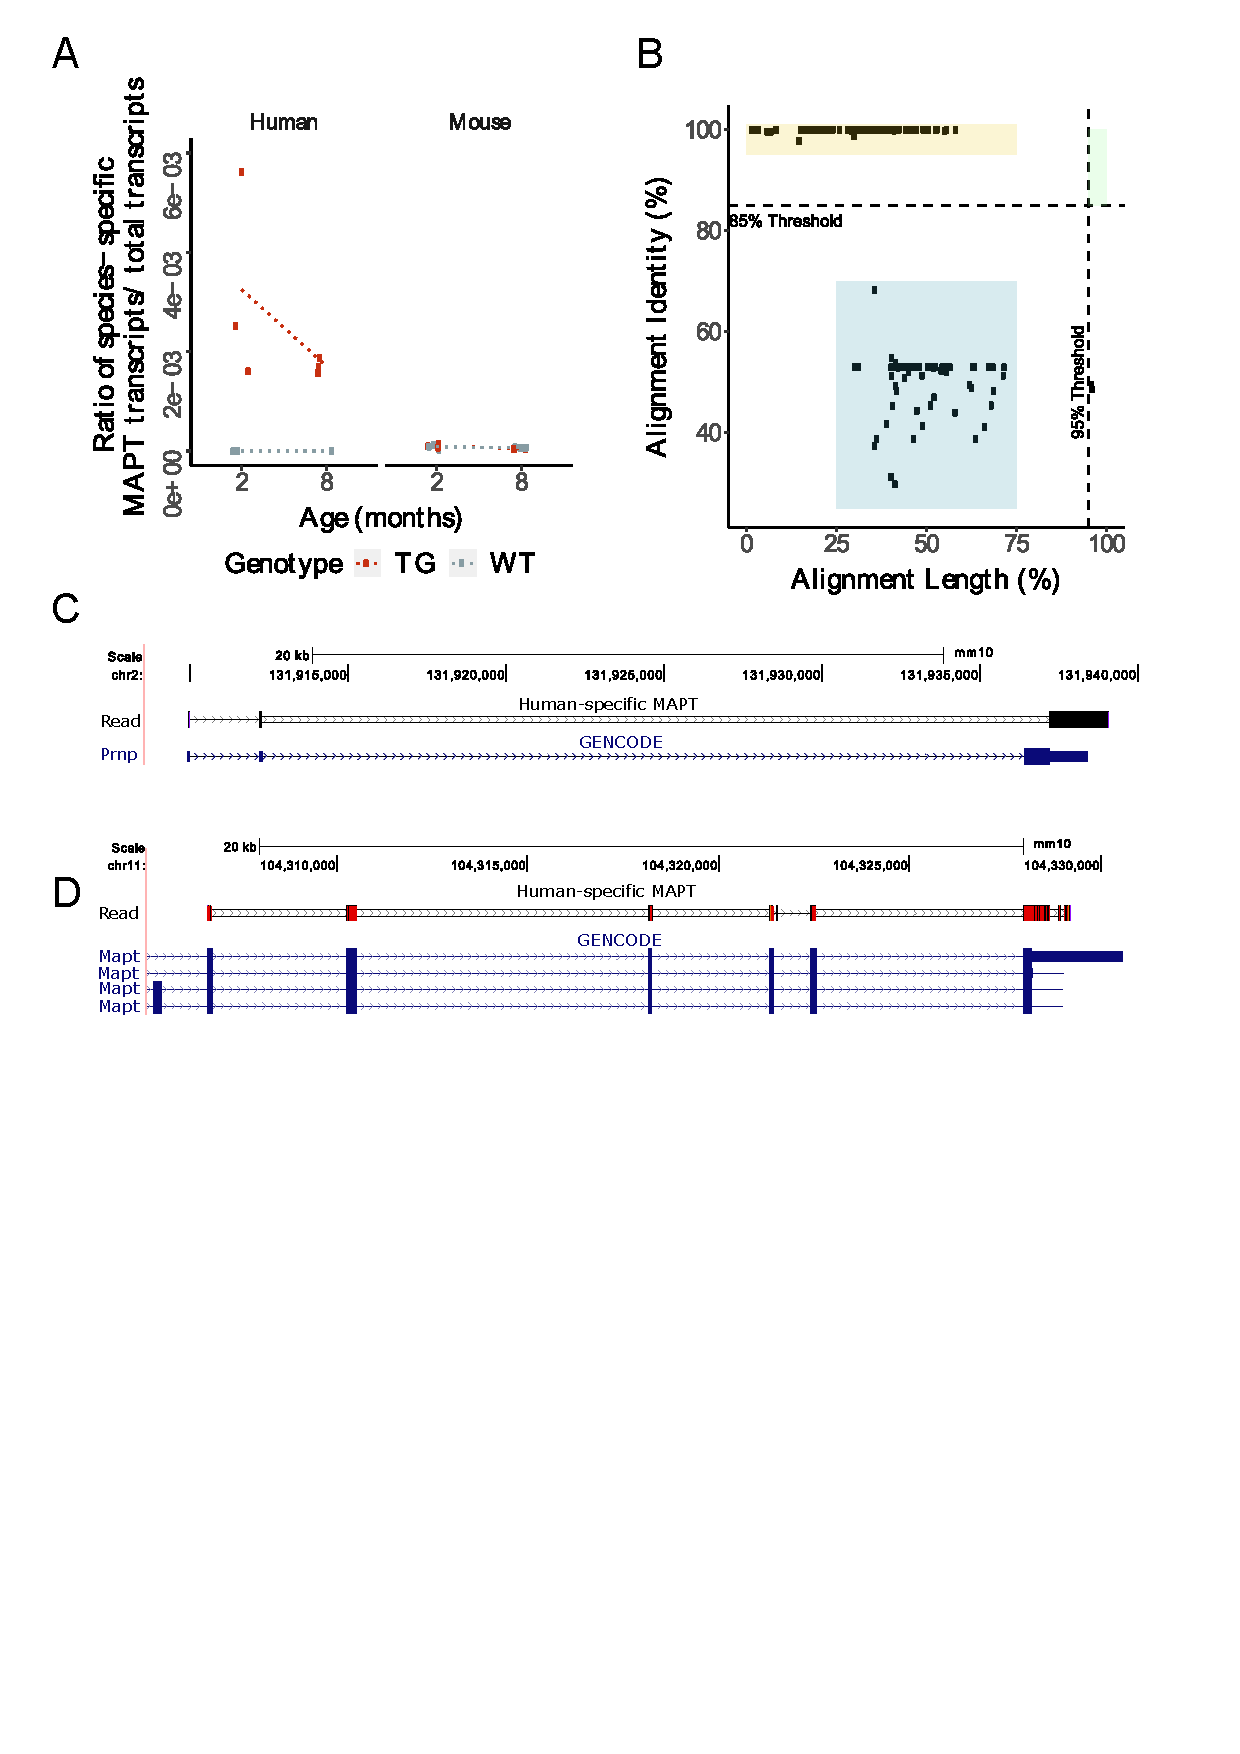
\includegraphics[page=1,trim={1cm 20cm 0cm 0cm},clip,scale = 0.55]{Figures/AltFigures_Diff.pdf}
	\end{center}
	\captionsetup{width=0.95\textwidth}
	\caption[Quantifying human-specific and mouse-specific \textit{MAPT}/\textit{Mapt} sequences in Iso-Seq Whole Transcriptome]%
	{\textbf{Human-specific \textit{MAPT} sequences only present in transgenic mice with poor alignment to mouse \textit{Prnp} and \textit{Mapt} gene}: Presence of human- and mouse-specific \textit{MAPT}/\textit{Mapt} sequences was determined in full-length transcripts generated from Iso-Seq merged dataset. \textbf{a)} Ratio of full-length transcripts that were mapped to human-specific \textit{MAPT} and mouse-specific \textit{Mapt} sequences. Dotted lines represent the mean paths across ages. \textbf{b)} As expected, human-specific \textit{MAPT} transcripts were poorly aligned to mouse genome. Transcripts were either aligned to mouse \textit{Prnp} gene (boxed yellow) or  mouse \textit{Mapt} gene (boxed blue). Alignment to mouse \textit{Prnp} gene was near 100\% within a short region, given that the transgene contains exon 2 and 3 of mouse \textit{Prnp} gene\cite{Ramsden2005}. Conversely, while human-specific \textit{MAPT} gene was sufficiently divergent from mouse \textit{Mapt} gene for transgene quantification, it still mapped to the mouse \textit{Mapt} gene 3'UTR albeit poorly. \textbf{c)} USCS genome browser tracks of human-specific (black) \textit{MAPT} transcripts (transgene) and mouse \textit{Prnp} gene and \textbf{d)} mouse \textit{Mapt} gene. Blue tracks represent known transcripts from reference mouse genome (mm10). Tracks were cropped and modified to remove irrelevant genes within the same locus.  UTR - Untranslated region}
	\label{fig:isoseq_humanmapt}
\end{figure}


\subsection{Transcriptome Annotation}
%No difference was observed in the number of transcripts generated between WT and TG (n = 12, two-tailed unpaired t-test, t = -0.005, df = 10, P = 0.996) or by age (n = 12, t = -1.58, df = 10, P = 0.15).
While identifying widespread RNA isoform diversity amongst genes expressed in the mouse entorhinal cortex (described in \cref{ch: whole_transcriptome}), no difference was observed in the number of genes (mean number = 13,302 genes) or isoforms (mean number = 35,157 isoforms) detected between wild-type and transgenic mouse at the two ages (WT: n = 6, TG: n = 6). Further characterisation of the transcriptome revealed similar profile of isoform diversity between the two phenotypes and ages (\cref{tab:isoseq_whole_subsqantioutput}), with half of the isoforms annotated as known (mean number = 18,567 isoforms (52.8\%), as also shown in \cref{sec:whole_novelIso}) and with a similar distribution in isoform length and number of exons (median: 9, range = 1-89) 

\begin{landscape}
	\begin{table}[]
		\centering
		\captionsetup{width=0.95\linewidth}
		\resizebox{1.5\textwidth}{!}{%
	\begin{tabular}{@{}ccccccc@{}}
		\toprule
		& \begin{tabular}[c]{@{}c@{}}wild-type \\ (n = 6)\end{tabular}              & \begin{tabular}[c]{@{}c@{}}Transgenic\\  (n = 6)\end{tabular}            & \begin{tabular}[c]{@{}c@{}}wild-type, 2 months \\ (n = 3)\end{tabular}    & \begin{tabular}[c]{@{}c@{}}wild-type, 8 months\\  (n = 3)\end{tabular}   & \begin{tabular}[c]{@{}c@{}}Transgenic, 2 months \\ (n = 3)\end{tabular}  & \begin{tabular}[c]{@{}c@{}}Transgenic, 8 months \\ (n = 3)\end{tabular}  \\ \midrule
		Total Number of Genes               & 14083                                                                    & 14183                                                                    & 12798                                                                    & 12947                                                                   & 12384                                                                    & 13418                                                                    \\
		Annotated Genes                     & 13911 (98.78\%)                                                          & 14018 (98.84\%)                                                          & 12696 (99.2\%)                                                           & 12816 (98.99\%)                                                         & 12286 (99.21\%)                                                          & 13289 (99.04\%)                                                          \\
		Novel Genes                         & 172 (1.22\%)                                                             & 165 (1.16\%)                                                             & 102 (0.8\%)                                                              & 131 (1.01\%)                                                            & 98 (0.79\%)                                                              & 129 (0.96\%)                                                             \\
		Total Number of Isoforms            & 41081                                                                    & 41671                                                                    & 31407                                                                    & 32630                                                                   & 28982                                                                    & 35169                                                                    \\
		FSM                                 & 18287 (44.51\%)                                                          & 18574 (44.57\%)                                                          & 15503 (49.36\%)                                                          & 15870 (48.64\%)                                                         & 14675 (50.63\%)                                                          & 16892 (48.03\%)                                                          \\
		ISM                                 & 3164 (7.7\%)                                                             & 3242 (7.78\%)                                                            & 2243 (7.14\%)                                                            & 2368 (7.26\%)                                                           & 2066 (7.13\%)                                                            & 2590 (7.36\%)                                                            \\
		NIC                                 & 11781 (28.68\%)                                                          & 12033 (28.88\%)                                                          & 8356 (26.61\%)                                                           & 8856 (27.14\%)                                                          & 7518 (25.94\%)                                                           & 9805 (27.88\%)                                                           \\
		NNC                                 & 7354 (17.9\%)                                                            & 7343 (17.62\%)                                                           & 4980 (15.86\%)                                                           & 5175 (15.86\%)                                                          & 4427 (15.27\%)                                                           & 5520 (15.7\%)                                                            \\
		Genic Genomic                       & 55 (0.13\%)                                                              & 54 (0.13\%)                                                              & 37 (0.12\%)                                                              & 41 (0.13\%)                                                             & 28 (0.1\%)                                                               & 43 (0.12\%)                                                              \\
		Antisense                           & 93 (0.23\%)                                                              & 100 (0.24\%)                                                             & 49 (0.16\%)                                                              & 74 (0.23\%)                                                             & 65 (0.22\%)                                                              & 74 (0.21\%)                                                              \\
		Fusion                              & 253 (0.62\%)                                                             & 242 (0.58\%)                                                             & 180 (0.57\%)                                                             & 176 (0.54\%)                                                            & 155 (0.53\%)                                                             & 177 (0.5\%)                                                              \\
		Intergenic                          & 94 (0.23\%)                                                              & 83 (0.2\%)                                                               & 59 (0.19\%)                                                              & 70 (0.21\%)                                                             & 48 (0.17\%)                                                              & 68 (0.19\%)                                                              \\
		Genic Intron                        & 0 (0\%)                                                                  & 0 (0\%)                                                                  & 0 (0\%)                                                                  & 0 (0\%)                                                                 & 0 (0\%)                                                                  & 0 (0\%)                                                                  \\
		Isoform Length (bp)                 & \begin{tabular}[c]{@{}c@{}}Median: 2946, \\ Range: 83-15016\end{tabular} & \begin{tabular}[c]{@{}c@{}}Median: 2955, \\ Range: 83-15913\end{tabular} & \begin{tabular}[c]{@{}c@{}}Median: 2987, \\ Range: 88-15016\end{tabular} & \begin{tabular}[c]{@{}c@{}}Median: 2890,\\ Range: 83-14850\end{tabular} & \begin{tabular}[c]{@{}c@{}}Median: 2798, \\ Range: 88-14302\end{tabular} & \begin{tabular}[c]{@{}c@{}}Median: 3013, \\ Range: 83-15913\end{tabular} \\
		Number of Exons                     & \begin{tabular}[c]{@{}c@{}}Median: 9, \\ Range: 1-89\end{tabular}        & \begin{tabular}[c]{@{}c@{}}Median: 9, \\ Range: 1-89\end{tabular}        & \begin{tabular}[c]{@{}c@{}}Median: 9, \\ Range: 1-89\end{tabular}        & \begin{tabular}[c]{@{}c@{}}Median: 9, \\ Range: 1-89\end{tabular}       & \begin{tabular}[c]{@{}c@{}}Median: 9, \\ Range: 1-77\end{tabular}        & \begin{tabular}[c]{@{}c@{}}Median: 9, \\ Range: 1-89\end{tabular}        \\
		Number of Isoforms within 50bp CAGE & 34574 (84.16\%)                                                          & 35097 (84.22\%)                                                          & 26539 (84.5\%)                                                           & 27689 (84.86\%)                                                         & 24398 (84.18\%)                                                          & 29911 (85.05\%)                                                          \\ \bottomrule
			\end{tabular}%
		}
	\caption[Overview of the whole transcriptome Iso-Seq datasets generated from mouse rTg4510, subsected by phenotype and age]%
	{Overview of the whole transcriptome Iso-Seq datasets generated from mouse rTg4510, subsected by phenotype and age. Annotations from wild-type (n = 6) and transgenic mouse (n = 6) were generated from merging Iso-Seq datasets from mouse aged 2 and 8 months of the respective phenotype. Novel genes refer to genes that were not currently present in existing genome annotations (mm10). Isoform can be further classified as known (FSM, ISM) or novel (ISM, NIC, NNC, Genic Genomic, Antisense, Fusion, Intergenic, Genic Intron), as described in \cref{sec:sq_exp}. FSM – Full Splice Match, ISM – Incomplete Splice Match, NIC – Novel In Catalogue, NNC – Novel Not in Catalogue.}
	\label{tab:isoseq_whole_subsqantioutput}
		\end{table}
\end{landscape}

\subsection{Alternative Splicing and Functional Diversity}
Transcriptome profiling of the mouse cortex previously identified widespread isoform diversity, driven predominantly by the usage of alternative first exons (AF) and exon skipping (ES) (described in \cref{sec:whole_novelIso}). Upon further examination, there was no significant difference in splicing patterns associated with rTg510 pathology or across age with AF (mean n = 20,400, 40.2\%) as the most prevalent event across all datasets \cref{AS_WholeTranscriptome_diff}. 
%stats?
%XX of known transcripts were identified to have intron retention; XX of known transcripts were identified to be fusion genes. XX of know transcripts identified to have non-sense-mediated decay. 

\vspace{0.5cm}
\begin{table}[!htp]
	\centering
	\captionsetup{width=1\textwidth}
	\caption[Alternative Splicing Events associated with tau pathology and age]%
	{\textbf{Alternative Splicing Events associated with tau pathology and age}. Tabulated is the number of splicing events detected for wild-type and transgenic Tg4510 mice aged 2 and 8 months (n = 12, 3 biological replicates per group)}
	\begin{tabular}{@{}ccccc@{}}
		\toprule
		\multirow{2}{*}{Splicing Events} & \multicolumn{2}{c}{wild-type} & \multicolumn{2}{c}{Transgenic} \\ \cmidrule(l){2-5} 
		& 2 months        & 8 months        & 2 months        & 8 months        \\ \midrule
		A3 & 3394 (6.8\%)    & 3526 (6.82\%)   & 2969 (6.41\%)   & 3825 (6.93\%)   \\
		A5 & 1388 (2.78\%)   & 1456 (2.82\%)   & 1231 (2.66\%)   & 1568 (2.84\%)   \\
		AF & 20185 (40.44\%) & 20597 (39.87\%) & 19182 (41.41\%) & 21781 (39.44\%) \\
		AL & 15620 (31.3\%)  & 16079 (31.12\%) & 14796 (31.94\%) & 16932 (30.66\%) \\
		IR & 3669 (7.35\%)   & 4169 (8.07\%)   & 3017 (6.51\%)   & 4794 (8.68\%)   \\
		MX & 324 (0.65\%)    & 315 (0.61\%)    & 285 (0.62\%)    & 378 (0.68\%)    \\
		SE & 5329 (10.68\%)  & 5524 (10.69\%)  & 4847 (10.46\%)  & 5953 (10.78\%)  \\ \bottomrule
	\end{tabular}
	\label{AS_WholeTranscriptome_diff}
\end{table}

However, aside from changes in splicing patterns, variations in structural and feature elements annotated across RNA and protein isoforms of the same gene can also have functional implications \cite{DeLaFuente2020}. Using \textit{TappAS}\cite{DeLaFuente2020}, we qualitatively catalogued the functional diversity of all multi-isoform genes, performing pairwise comparisons between isoforms of the same gene to test for either the i) presence or absence of the annotated feature or ii) in the annotated genomic positions (a feature is classified as varying if the feature's coordinates differ by >9bp between isoforms of the same gene). Of note, many of the protein-defined features can be explored using both approaches given that these elements can be affected through complete skipping (resulting in absence) or partial disruption (resulting in varied genomic position).

Under these two approaches, we identified that the majority of genes had elements that varied either by absence/presence or by position (\cref{fig:FDA_whole}\textbf{a}). Among elements at a transcript level, miRNA binding had the highest rate of varying (n = 4209 genes) with a large number of miRNA sites varying at the 3'UTR (n = 431). Top miRNAs included miR-207 (P = 0.0003, Adjusted P = 0.07, Varying n = 163 genes), which transfected expression in astrocytes was found to alleviate symptoms of depression in stressed mice\cite{Li2020}, and miR-335-3p (P = 0.0015, Adjusted P = 0.1992, Varying n = 167 genes), which was found enriched in aged cultured astrocytes and hippocampal brains\cite{Raihan2018}, while downregulated in PD patients versus controls\cite{Oliveira2020}. 
%nonsense-mediated decay had no variation
Regarding protein-level features, PFAM domains had the highest rate of varying (55\%), with cytochrome P450 as the top most varying PFAM domain (n = 10 genes, P = 0.002) and protein kinase domain as the domain with most varied number of genes (n = 126 genes, P = 0.0095). GO analysis of these genes where protein kinase domain varied across isoforms identified significant enrichment for the MAPK (Odds ratio = 21.06, Adjusted P = 5.45 x 10\textsuperscript{-23}) and Neurotrophin signalling pathway (Odds ratio = 40.36, Adjusted P = 6.711 x 10\textsuperscript{-23}). 

Poly A site had the highest rate of varying by position among transcript-level features (90.2\% across 7,647 genes), followed by coding squence (80.3\% across 6,812 genes). Furthermore, the vast majority of UTR-varying genes also exhibited CDS variation (\cref{fig:FDA_whole}\textbf{c}). This included \textit{Celf2} (\cref{fig:Celf}), which was identified as exhibiting varying lengths of 5'UTR, 3'UTR and polyA in combination with varying miRNA binding sites. The top PFAM domain by position was Ras family (P = 0.0001, Adjusted P = 0.38, Varying n = 58 genes). 

\begin{figure}[!htp]
	\centering
	\includegraphics[page=2,trim={3cm 7cm 3cm 4cm},scale = 0.6]{Figures/WholeFDA.pdf}
	\captionsetup{width=0.95\textwidth}
	\caption[Variation in functional elements annotated across RNA and protein isoforms]%
	{\textbf{Variation in functional elements annotated across RNA and protein isoforms} XXX}   
	\label{fig:FDA_whole}
\end{figure}


\begin{figure}[!htp]
	\centering
	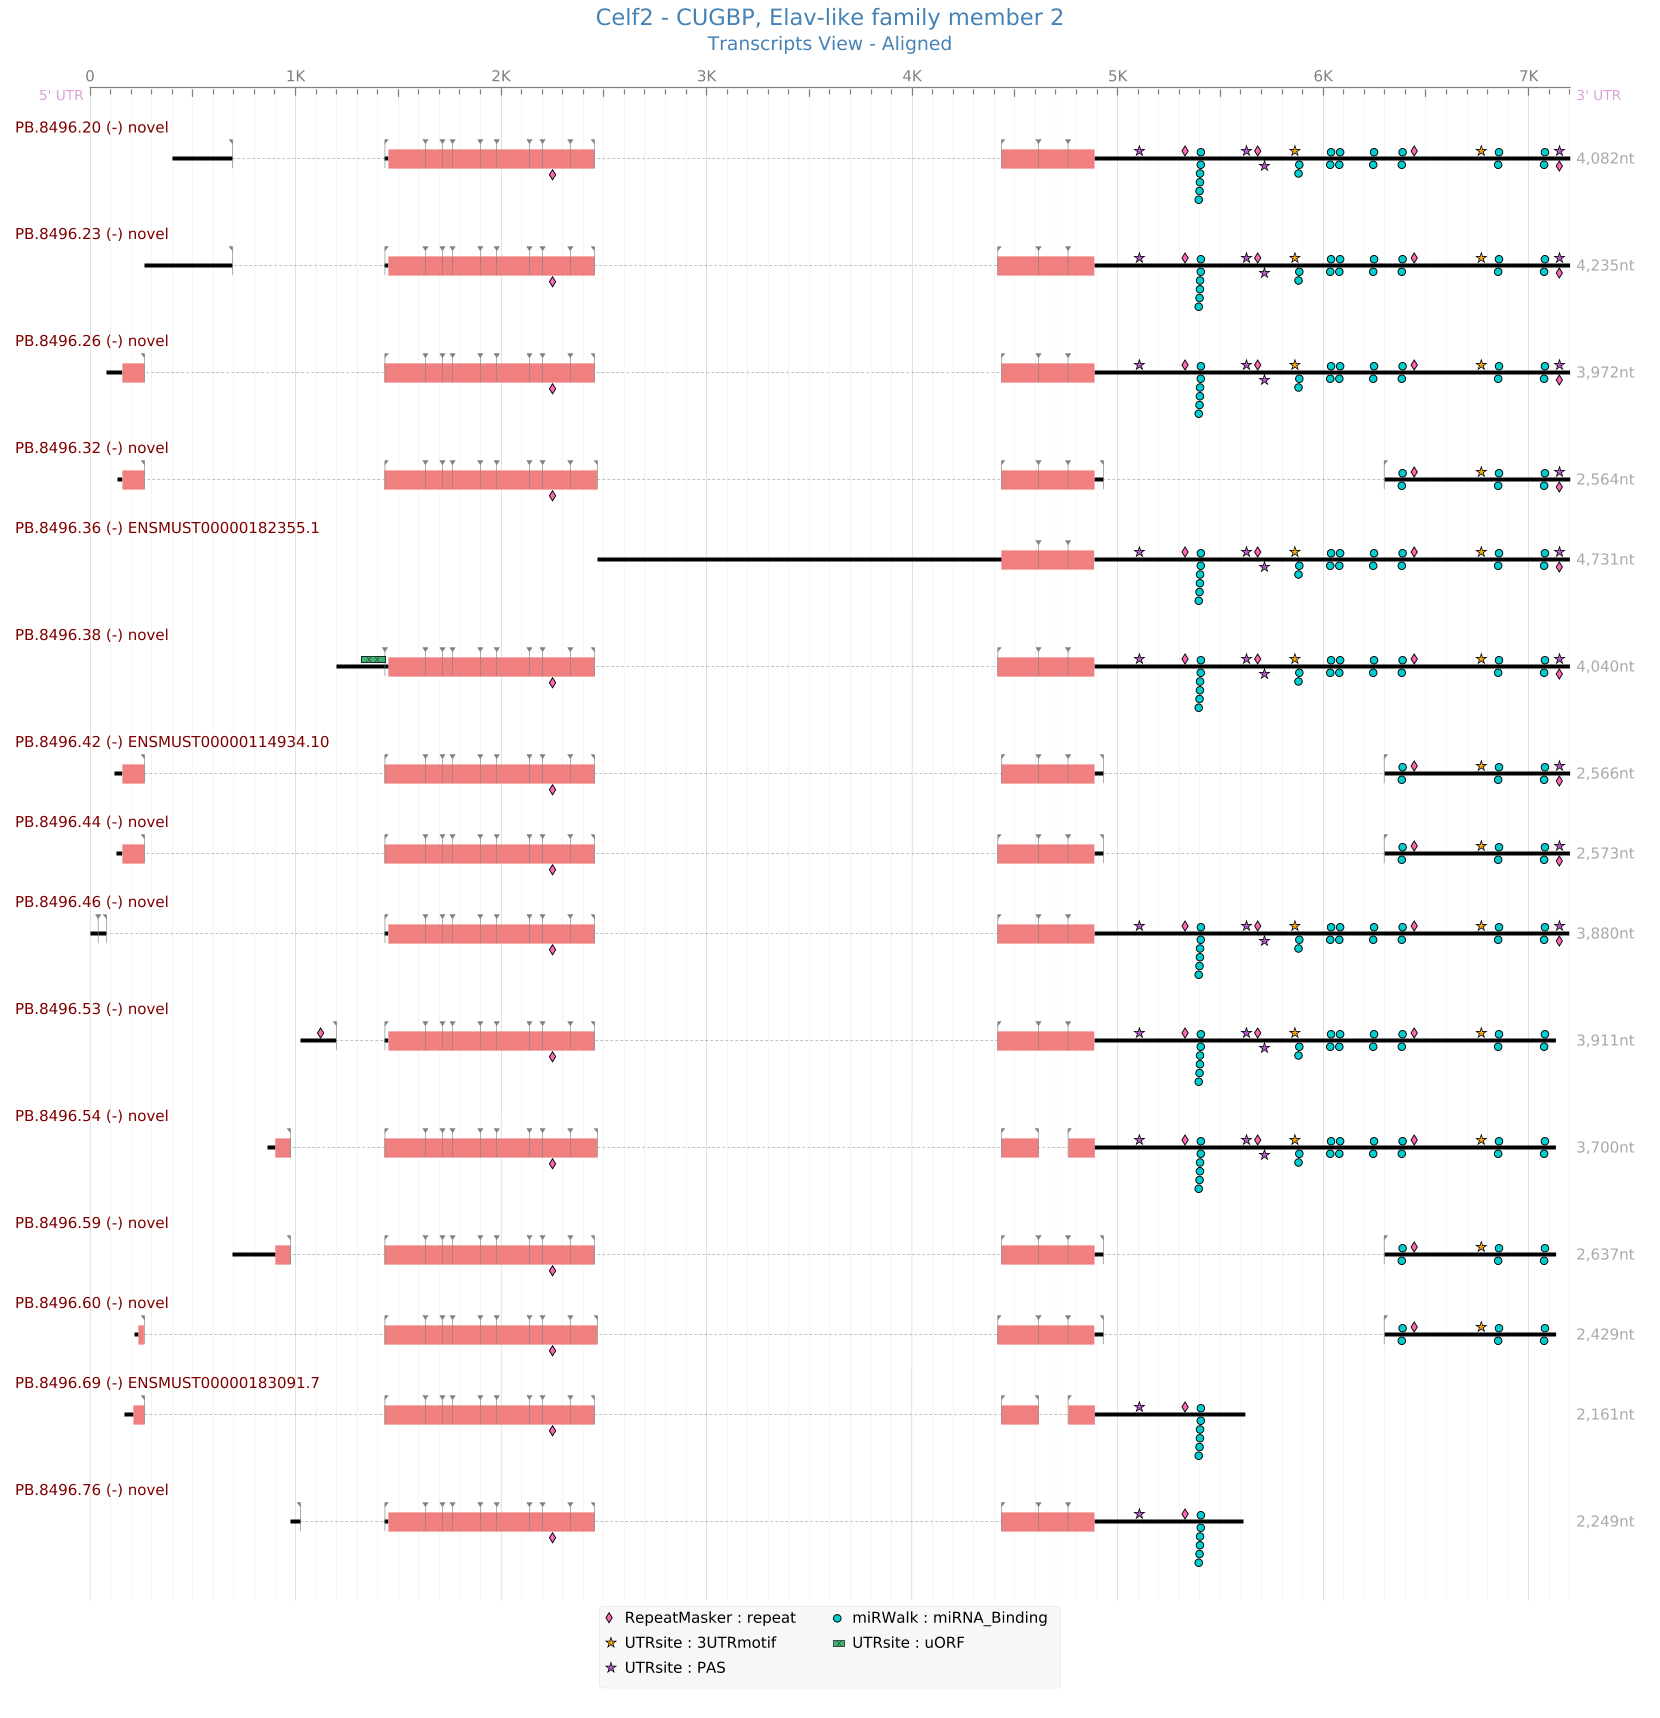
\includegraphics[scale = 0.3]{Figures/tappAS_Celf2.png}
	\captionsetup{width=0.95\textwidth}
	\caption[Varying functinonal elements in isoforms associated with \textit{Celf2}]%
	{\textbf{Varying functinonal elements in isoforms associated with \textit{Celf2}}.\textit{TappAS} graphical representation of the transcript-level annotation for \textit{Celf2}, where 5'UTR, 3'UTR, CDS, and 3' alternative polyadenylation variation were detected.}   
	\label{fig:Celf}
\end{figure}	



\clearpage 
\subsection{Differential Gene Expression Analysis}
Our group previously characterised widespread transcriptional differences in rTg4510 entorhinal cortex, identifying extensive differences in gene expression associated with development of tau pathology in TG mice (n = 154 differentially expressed genes)\cite{Castanho2020}. Mapping the same RNA-Seq reads (n = 29 TG, n = 30 WT) to Iso-Seq reads (n = 6 TG, n = 6 WT) derived from the same animals rather to the reference genome annotation, we similarly identify extensive differences in gene expression (n = XX differentially expressed genes) with a large overlap. 

The hybrid approach also enabled identification of tau-pathology associated changes in genes not previously known in reference. Using the Iso-Seq reads as annotation and RNA-Seq reads for expression, we identified robust expression changes in a few genes (n = 3) that we would have otherwise not detected if we used the reference genome for annotation. These "novel" genes, not present in existing genome annotations (mm10), have been previously characterised as more lowly-expressed and often were antisense to known genes, with a large proportion sharing exonic regions either at the 5'UTR, 3'UTR or within the gene body (\cref{sec:whole_novelgenes}). The most significant differentially-expressed novel gene was identified in Chromosome 10 (\cref{fig:whole_novelgene_difftracks}\textbf{a}), with progressive down-regulation in TG over time (\cref{fig:whole_novelgene_diffexp}\textbf{a}). The other differentially-expressed novel genes were found antisense to \textit{Fgfr1op} (\cref{fig:whole_novelgene_difftracks}\textbf{b}), within the gene-body, and to \textit{Htra1}  (\cref{fig:whole_novelgene_difftracks}\textbf{c}), at the 5'UTR. Both genes were associated with increased expression in TG compared to the WT over time (\cref{fig:whole_novelgene_diffexp}\textbf{b,d}). Notably, while \textit{Fgfr1op} was not identified as differentially-expressed (\cref{fig:whole_novelgene_diffexp}\textbf{c}), \textit{Htra1} was also found to have higher expression in TG compared to WT (\cref{fig:whole_novelgene_diffexp}\textbf{e}).     
%Htra1-AS shared exonic regions with Htra1 so misalignment of RNA-Seq reads

\begin{landscape}
	\begin{figure}[!htp]
		\centering
		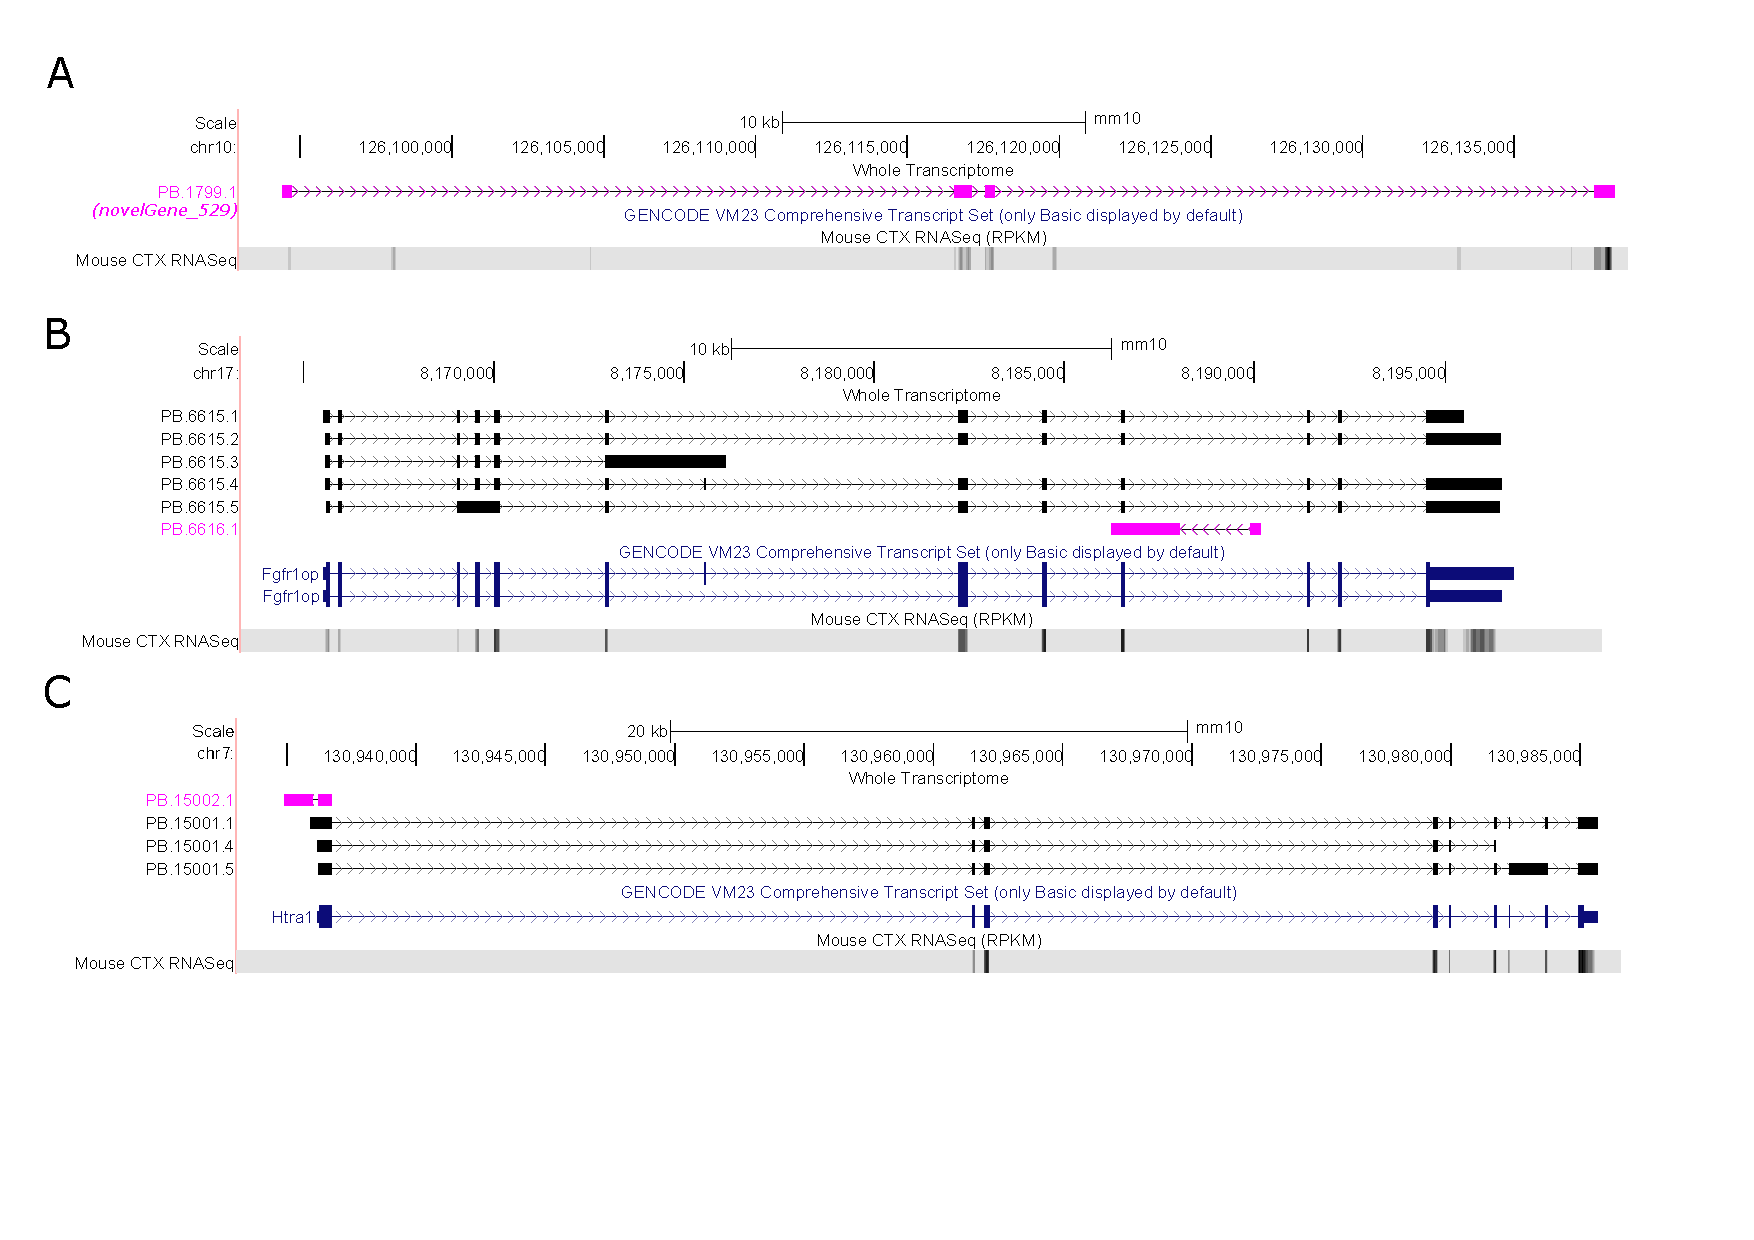
\includegraphics[page=1,trim={0 4cm 0 0}, scale = 0.45]{Figures/TracksFigures_Diff.pdf}
		\captionsetup{width=1.4\textwidth}
		\caption[Tracks of novel genes that were differentially expressed in rTg4510 mice]%
		{\textbf{Tracks of novel genes that were differentially expressed in rTg4510 mice}: Shown are UCSC genome browser Iso-Seq tracks of three novel genes - \textbf{a)}novel gene in Chromosome 10, \textbf{b)} novel gene antisense to \textit{Fgfr1op}, and \textbf{c)} novel gene antisense to \textit{Htra1} - that were identified as differentially expressed with Iso-Seq reads (n = 12 samples) as annotation and RNA-Seq reads (n = 59 samples) as expression. The isoforms were coloured based on \textit{SQANTI} classification, with the novel gene coloured grey for genic/intergenic in panel a) and pink for antisense in panels b) and c). Shown are also the reference genome annotations (mm10) and RNA-Seq reads.}   
		\label{fig:whole_novelgene_difftracks}
	\end{figure}
\end{landscape}

\begin{figure}[!htp]
	\begin{center}
		\includegraphics[page=11,scale = 0.55]{Figures/WholeDifferentialAnalysis.pdf}
	\end{center}
	\captionsetup{width=0.95\textwidth}
	\caption[Comparison of Known and Novel Isoforms from Iso-Seq Whole Transcriptome runs]%
	{\textbf{Novel isoforms were less expressed, longer and had more exons than known isoforms}: Shown is the \textbf{a)}}   
	\label{fig:whole_novelgene_diffexp}
\end{figure}
   

%\boldheader{Usage of Iso-Seq reads alone detected robust changes in gene expression}
While Iso-Seq reads are commonly used for accurately characterising RNA diversity, we found that Iso-Seq reads were also able to accurately quantify the abundance of highly-expressed transcripts - as illustrated by the strong correlation of gene-level expression quantified using Iso-Seq and RNA-Seq reads, and near-perfect correlation Iso-Seq reads and actual amount of ERCC controls (described in XX). Strikingly, despite the lower long-read sequencing coverage and smaller sample size (n = 6 TG, n = 6 WT) sequenced on the long-read platform, a significant number of genes (n = 446 genes) were identified as differentially expressed when we used the Iso-Seq long reads for both annotation and expression. Using \textit{EnrichR}, differentially expressed genes (n = 466) were found to be highly enriched in lysosome (KEGG 2021 Human: odds ratio = 5.99, adjusted P = 4.41 x 10\textsuperscript{-6}) and in particularly the TGF-\textbeta pathway (WikiPathway 2021 Human: odds ratio = 58.98, adjusted P = 2.69 x 10\textsuperscript{-3} ). Classification of the differentially expressed genes by effects (depicted in \cref{fig:dea_model} and showcased in \cref{fig:dea_model_genexp}), further identified the majority (n = 340 genes, \cref{fig:dea_model_num}) to be associated with tau pathology (n = 23, \cref{fig:dea_model_genexp}\textbf{a}) and progressive with age (n = 340, \cref{fig:dea_model_genexp}\textbf{d,e,f,g}).       
 
\begin{figure}[h]
	\centering
	\includegraphics[page=5,trim={0 20cm 0 0},clip,scale = 0.55]{Figures/WholeDifferentialAnalysis.pdf}
	\captionsetup{width=0.95\textwidth}
	\caption[Differentially expressed genes classified by conditions]%
	{\textbf{Differentially expressed genes were identified across all the different conditions, with most genes exhibiting an interaction effect of rTg4510 genotype and age} Shown is a bar plot of the number of differentially expressed genes (n = 446) classified by the different conditions, as modelled in \cref{fig:dea_model}. The differentially expressed genes were identified from the whole transcriptome datasets (WT = 6, TG = 6, across age 2 and 8 months) using Iso-Seq read counts as abundance. WT - wild-type, TG - Transgenic.}    
	\label{fig:dea_model_num}
\end{figure}

\begin{figure}[h]
	\centering
	\includegraphics[page=6,scale = 0.55]{Figures/WholeDifferentialAnalysis.pdf}
	\captionsetup{width=0.95\textwidth}
	\caption[Examples of gene expression differing across conditions]%
	{\textbf{Differential expressed genes exhibiting genotype, age and interaction effects} Shown are examples of differentially expressed genes classified under the different models, using the whole transcriptome dataset (WT = 6, TG = 6, across age 2 and 8 months) using Iso-Seq read counts as abundance: \textbf{a} \textit{Herc2} with a genotype effect, \textbf{b} \textit{Kcng1} with a genotype and age effect, \textbf{c} \textit{Clnc3} with an age effect, and \textbf{d} \textit{Cd34}, \textbf{e} \textit{Unc93b1}, \textbf{f} \textit{Csf1r} and \textbf{g} \textit{Gjb2} with an interaction effect. Dotted lines represent the mean paths across ages.}   
	\label{fig:dea_model_genexp}
\end{figure}

Usage of Iso-Seq reads alone identified differentially-expressed genes previously reported to be highly associated with AD. The top ranked tau-associated differentially-expressed genes that was found to be progressive with age in our previous analyse\cite{Castanho2020} was also recapitulated (\cref{fig:whole_dea}\textbf{a,b}): \textit{Gfap}, which encodes for glial fibrillary acidic protein (GFAP\nomenclature{GFAP}{Glial Fibrillary Acidic Protein}), a cytoskeletal protein that acts as a marker for astrocyte activation and proliferation - its increased expression was reported to correlate with increased neurofibrillary tangles density in Alzheimer's disease entorhinal cortex tissues \cite{Muramori1998}. Higher GFAP levels have also be documented in cerebrospinal fluid (CSF) in patients with AD compared to healthy control \cite{Ishiki2016}, and more recently, in plasma of cognitively intact older adults at risk of AD \cite{Chatterjee2021}. 


\begin{figure}[h]
	\begin{center}
		\includegraphics[page=2,scale = 0.55]{Figures/WholeDifferentialAnalysis.pdf}
	\end{center}
	\captionsetup{width=0.95\textwidth}
	\caption[Comparison of Known and Novel Isoforms from Iso-Seq Whole Transcriptome runs]%
	{\textbf{Novel isoforms were less expressed, longer and had more exons than known isoforms}: Shown is the \textbf{a)} Iso-Seq transcript expression, the \textbf{c)} transcript length, and the \textbf{e)} the number of exons of novel and known isoforms. The known and novel isoforms can be further subdivided and classified, with the \textbf{b)} Iso-Seq expression \textbf{d)} transcript length and \textbf{f)} number of exons for each category. According to SQANTI, known isoforms are subdivided into FSM and ISM, and novel isoforms are subdivided into NIC, NNC, and fusion. FSM – Full Splice Match, ISM – Incomplete Splice Match, NIC – Novel In Catalogue, NNC – Novel Not in Catalogue.}   
	\label{fig:whole_dea}
\end{figure}


Other top-ranked differentially-expressed genes have been reported to be involved in AD development and pathology, notably \textit{C4b} - a member of the complement immune system (\cref{fig:whole_dea}\textbf{c,d}), \textit{Slc14a1} encoding the urea transporter 1, \textit{Tgfbr1} encoding the TGF-\textbeta receptor protein (\cref{fig:whole_dea}\textbf{e,f}) and \textit{Unc93b1}, a transmembrane protein required for toll (\cref{tab:dea_wholemouse}). Up-regulated expression of these genes have been observed previously in AD patients and other AD mouse models \cite{Zorzetto2016,Castillo2017,Wirz2013}. 

%log2fc calculated by mean expression at 8 case/mean expression at 8 control
\begin{table}[!htp]
	\centering
	\begin{tabularx}{0.96\textwidth}{cccccccc}
		\toprule
		\multirow{3}{*}{Gene} & \multirow{3}{*}{FDR} & \multirow{3}{*}{R\textsuperscript{2}} & \multirow{3}{*}{\begin{tabular}[c]{@{}c@{}}log2-fold \\ change \\ (8 months)\end{tabular}} & \multicolumn{4}{c}{Mean Gene Expression}                      \\ \cmidrule(l){5-8} 
		&                      &                    &                                                                                            & \multicolumn{2}{c}{wild-type} & \multicolumn{2}{c}{Transgenic} \\ \cmidrule(l){5-8} 
		&                      &                    &                                                                                            & 2 months      & 8 months     & 2 months       & 8 months      \\ \midrule
		\textit{C4b}          & 3.9E-39              & 0.941              & 4.44                                                                                       & 3.57          & 1.79         & 4.03           & 87.4          \\
		\textit{Gfap}         & 8.88E-36             & 0.935              & 3.09                                                                                       & 75.6          & 62.3         & 106            & 900           \\
		\textit{Tgfbr1}       & 1.06E-20             & 0.880              & 3.48                                                                                       & 0.673         & 3.39         & 1.28           & 14.4          \\
		\textit{Slc14a1}      & 1.94E-16             & 0.872              & 2.92                                                                                       & 8.56          & 12.3         & 5.2            & 39.4          \\
		\textit{Unc93b1}      & 1.69E-15             & 0.853              & 1.5                                                                                        & 3.68          & 5.04         & 6.68           & 18.9          \\ \bottomrule
	\end{tabularx}
	\caption[Top-ranked differentially expressed genes associated with rTg4510]%
	{Tabulated are the top-ranked genes identified as differentially expressed in rTg4510 using \textit{maSigPro} with Iso-Seq defined transcriptome for annotation and Iso-Seq FL read count as expression. Gene expression is determined from the sum of normalised expression of associated transcripts. FDR - False Discovery Rate. }
	\label{tab:dea_wholemouse}
\end{table}




\clearpage
\subsection{Differential Isoform Expression Analysis}
One of the added advantages of long reads over short-reads is the power to accurately identify isoforms and to explore isoform expression changes across conditions and over time. Using \textit{MaSigPro} with Iso-Seq reads as both reference annotation and expression, we identified hundreds of differentially expressed isoforms (n = 582 isoforms), of which 36 isoforms (6.19\%) were associated with rTg4510 genotype, and 378 isoforms (64.9\%) associated with progressive tau pathology. 

\boldheader{Robust changes in isoform expression associated with progressive tau pathology were identified with Iso-Seq annotation and expression}
Strikingly, the two most significant progressive-tau-associated differentially expressed isoforms were annotated to \textit{Gfap} (\cref{fig:DEI_gfap}) and \textit{C4b} (\cref{fig:DEI_c4b}), the top two most differentially-expressed genes (\cref{tab:dea_wholemouse}). Both genes were characterised by a dominant known isoform in rTg4510 mice, which was significantly up-regulated with progressive tau pathology (\cref{fig:DEI_gfap}\textbf{a}, \cref{fig:DEI_c4b}\textbf{a}), indicating that increased \textit{Gfap} (\cref{fig:whole_dea}\textbf{a}) and \textit{C4b} (\cref{fig:whole_dea}\textbf{c}) gene expression in rTg4510 mice were primarily driven by one associated isoform. Notably, expression of other minor novel isoforms was also higher in rTg4510 mice aged 8 months (\cref{fig:DEI_gfap}\textbf{b}, \cref{fig:DEI_c4b}\textbf{b}). A similar finding was also observed when using RNA-Seq reads as abundance, though tau-pathology associated expression changes in minor isoforms were significantly more pronounced - a reflection of the comparably higher sequencing coverage of RNA-Seq reads to Iso-Seq reads. 

Other isoforms that were significantly unregulated with progressive tau pathology were annotated to genes that have been previously strongly implicated in AD pathology and development (\cref{fig:DEI_ADgenes_isoseq}). This included ENSMUST00000151120.8 associated with \textit{Ctsd}, which encodes for Cathepsin D, a lysosomal protease that is involved in degradation of A$\beta$ \cite{JR1996}, tau \cite{A1997}, and has recently been identified as a key regulator of A$\beta$42/40 ratio \cite{Suire2020}. Other isoforms include ENSMUST00000172785.7 associated with \textit{H2-D1} - that encodes for major histocompatibility complex (MHC) class 1, an immune-related gene that has been found to be upregulated in microglial cells of a different mouse model of neurodegeneration with AD-like phenotypes \cite{Mathys2017} - ENSMUST00000028624.8 associated with \textit{Gatm}, a mitochondrial protein that has been recently revealed as a key protein signature of AD from a large proteomic analysis of human cortex and CSF \cite{Wang2020}, - and ENSMUST00000030765.6 associated with \textit{Padi2}/\textit{Pad2}, an enzyme that has been found abnormally activated in astrocytes of patients with AD \cite{A2005}.

\boldheader{Iso-Seq reads can accurately quantify highly-expressed isoforms and identify significant expression changes in isoforms annotated to highly-expressed genes}
Observations of differential isoform expression using Iso-Seq reads as expression were recapitulated with RNA-Seq reads, highlighting the power to accurately quantify isoforms at high expression (\cref{fig:DEI_ADgenes_rnaseq}).
However, on closer examination, the majority of isoforms identified as differentially expressed with progressive tau pathology (n = 321, 84.9\%) were not similarly identified as differentially expressed when RNA-Seq reads were used as expression. Given that the wide majority of Iso-Seq-identified-differentially-expressed isoforms were very-lowly expressed (295 isoforms,91.9\%, with mean full-length counts < 24 FL, n = 12 samples) with low read count, a seemingly significant expression change may result in calling the isoform differentially expressed (\cref{fig:dei_lowisoexp}). However, even for more highly-expressed isoforms, while a change in mean expression was observed, the variance was substantial due to a small sample size (n = 3 replicates). Conversely, with a greater sample size (n = 6 replicates) and higher sequencing coverage of RNA-Seq reads, the usage of RNA-Seq reads as expression reduced the probability of calling an isoform as differentially expressed due to chance (\cref{fig:dei_highisoexp}).      

\begin{figure}[!htp]
	\centering
	\includegraphics[page=4,scale = 0.55]{Figures/WholeDifferentialAnalysis.pdf}
	\captionsetup{width=0.95\textwidth}
	\caption[Differential Isoform Expression: Changes in transcript expression of isoforms associated with \textit{Gfap}]%
	{\textbf{Significant upregulation of known isoform of \textit{Gfap} with progressive tau pathology}. Shown are \textbf{a)} normalised counts of \textit{Gfap} with associated isoforms in WT and TG across 2 time points (aged 2 and 8 months) for emphasis of dominant isoform (PB.2972.16, ENSMUST00000067444.9), and \textbf{b)} alternative plot of \textit{Gfap} with y-axis log-transformed for better visualisation of minor isoform expression. Novel minor isoforms, PB.2972.13 and PB.2972.14, were also identified as differentially expressed. Normalised counts of isoforms are derived directly from Iso-Seq full-length reads. FSM - Full Splice Match, ISM - Incomplete Splice Match, NIC - Novel In Catalogue, NNC - Novel Not in Catalogue. WT - Wild-type, TG - Transgenic. Dotted lines represent the mean paths across ages.} 
	\label{fig:DEI_gfap}
\end{figure}

\begin{figure}[!htp]
	\centering
	\includegraphics[page=12,scale = 0.55]{Figures/WholeDifferentialAnalysis.pdf}
	\captionsetup{width=0.95\textwidth}
	\caption[Differential Isoform Expression: Changes in transcript expression of isoforms associated with \textit{C4b}]%
	{\textbf{Significant upregulation of known isoform of \textit{C4b} with progressive tau pathology}. Shown are \textbf{a)} normalised counts of \textit{C4b} with associated isoforms in WT and TG across 2 time points (aged 2 and 8 months) for emphasis of dominant isoform (PB.7004.8, ENSMUST00000069507.8), and \textbf{b)} alternative plot of \textit{C4b} with y-axis log-transformed for better visualisation of minor isoform expression. Normalised counts of isoforms are derived directly from Iso-Seq full-length reads. FSM - Full Splice Match, ISM - Incomplete Splice Match, NIC - Novel In Catalogue, NNC - Novel Not in Catalogue. WT - Wild-type, TG - Transgenic. Dotted lines represent the mean paths across ages.}   
	\label{fig:DEI_c4b}
\end{figure}

\begin{figure}[!htp]
	\centering
	\includegraphics[page=18,scale = 0.55]{Figures/WholeDifferentialAnalysis.pdf}
	\captionsetup{width=0.95\textwidth}
	\caption[Robust changes in transcript expression of isoforms annotated to genes that are strongly implicated in AD]%
	{\textbf{Robust changes in transcript expression of isoforms annotated to genes that are strongly implicated in AD}. Using Iso-Seq reads (n = 6 WT, n = 6 TG, across 2 and 8 months) as annotation and expression, differential isoform expression was observed for \textbf{a)} ENSMUST00000151120.8 (PB.15108.6) annotated to \textit{Ctsd}, \textbf{b)} ENSMUST00000172785.7 (PB.7039.1) annotated to \textit{H2-D1}, \textbf{c)} ENSMUST00000028624.8 (PB.9298.1) annotated to \textit{Gatm}, and \textbf{d)} ENSMUST00000030765.6 (PB.11607.2) associated with \textit{Padi2}/\textit{Pad2}.  WT - wild-type, TG - Transgenic. Dotted lines represent the mean paths across ages.}    
	\label{fig:DEI_ADgenes_isoseq}
\end{figure}

\begin{figure}[!htp]
	\centering
	\includegraphics[page=19,scale = 0.55]{Figures/WholeDifferentialAnalysis.pdf}
	\captionsetup{width=0.95\textwidth}
	\caption[Changes in transcript expression of genes strongly implicated in AD were similarly detected using RNA-Seq reads]%
	{\textbf{Changes in transcript expression of genes strongly implicated in AD were similarly detected using RNA-Seq reads}. Usage of RNA-Seq reads (n = 30 WT, n = 29 TG, across 2, 4, 6 and 8 months) as expression similarly identified isoforms as differentially expressed (\cref{fig:DEI_ADgenes_isoseq}). \textbf{a)} ENSMUST00000151120.8 (PB.15108.6) annotated to \textit{Ctsd}, \textbf{b)} ENSMUST00000172785.7 (PB.7039.1) annotated to \textit{H2-D1}, \textbf{c)} ENSMUST00000028624.8 (PB.9298.1) annotated to \textit{Gatm}, and \textbf{d)} ENSMUST00000030765.6 (PB.11607.2) associated with \textit{Padi2}/\textit{Pad2}.  WT - Wild-type, TG - Transgenic. Dotted lines represent the mean paths across ages.}   
	\label{fig:DEI_ADgenes_rnaseq}
\end{figure}

\begin{figure}[!htp]
	\centering
	\includegraphics[page=15,scale = 0.55]{Figures/WholeDifferentialAnalysis.pdf}
	\captionsetup{width=0.95\textwidth}
	\caption[Differential isoform expressed observed with Iso-Seq reads as expression were not recapitulated using RNA-Seq reads]%
	{\textbf{Differential isoform expressed observed with Iso-Seq reads as expression were not recapitulated using RNA-Seq reads}. Shown are normalised counts \textbf{a)} \textit{Cd34} and \textbf{c)} \textit{Ubqln1} with associated isoforms identified from using Iso-Seq reads as expression, and of the same two genes \textbf{b)} \textit{Cd34} and \textbf{d)} \textit{Ubqln1} identified from using RNA-Seq reads as expression. Significant changes in isoform expression identified using Iso-Seq reads as expression - PB.1063.2 associated with \textit{Cd34} and PB.4255.13 and PB.4255.4 associated with \textit{Ubqln1} - was not recapitulated when using RNA-Seq reads as expression, due to lower sequencing coverage. Notably, minor isoforms had a higher expression with RNA-Seq alignment than direct detection with Iso-Seq reads.
	FSM - Full Splice Match, ISM - Incomplete Splice Match, NIC - Novel In Catalogue, NNC - Novel Not in Catalogue. Dotted lines represent the mean paths across ages.
	}   
	\label{fig:dei_lowisoexp}
\end{figure}

\begin{figure}[!htp]
	\centering
	\includegraphics[page=17,trim={0cm 20cm 0cm 0cm},clip,scale = 0.55]{Figures/WholeDifferentialAnalysis.pdf}
	\captionsetup{width=0.95\textwidth}
	\caption[Differential Isoform Expression observed in isoforms with high expression but large variance]%
	{\textbf{Usage of RNA-Seq reads as expression, with larger sample size, reduce probability of calling isoforms differentially expressed due to chance} Shown are \textbf{a)} \textit{Slc1a3} with associated isoforms identified as differentially expressed when Iso-Seq reads were used as expression (n = 6 WT, n = 6 TG, across 2 time points), and \textbf{b)} \textit{Slc1a3} when RNA-Seq reads were used as expression (n = 30 WT, n = 29 TG, across 4 time points). 
	\\
	\\	
	Using Iso-Seq reads as expression, the more-highly expressed isoforms PB.527.1 (red) in Figure a) was identified as differentially expressed. The expression change, however, of the same isoform was less prominent when RNA-Seq reads were used due to greater sample size and higher sequencing coverage. Notably, all the minor isoforms had a higher expression when RNA-Seq reads were used, resulting in some novel isoforms not being pre-filtered (as in the case with Iso-Seq reads as expression due to low full-length read count)
	\\
	\\
	FSM - Full Splice Match, ISM - Incomplete Splice Match, NIC - Novel In Catalogue, NNC - Novel Not in Catalogue. Dotted lines represent the mean paths across ages.
}   
	\label{fig:dei_highisoexp}
\end{figure}


\clearpage
\subsection{Differential Isoform Usage Analysis}
Contributing to the complexity of transcript regulation through alternative splicing, while the expression of a gene may be constant between conditions, the relative expression of the isoforms (and thus isoform proportion) can change. This phenomenon is known as differential transcript/isoform usage (DIU), and was also assessed using \textit{tappAS} for genes with more than one isoform. Of note, a major isoform switching event occurs when the dominant (major) isoform in one condition becomes a minor isoform in another.    

\boldheader{Usage of Iso-Seq reads results in many false positives due to insufficient sequencing depth}
Using Iso-Seq reads for annotation and expression and after filtering lowly-expressed isoforms, we identified 400 genes that were characterised with differential isoform usage. However upon further examination, the majority of these genes were lowly expressed and the associated isoforms that were observed to undergo differential usage had only 1-2 full-length long-read counts. We were therefore not confident in any of observed DIU changes detected with Iso-Seq abundance from the whole transcriptome sequencing due to low sequencing depth. Indeed, none of the DTU genes were significant after applying a gene expression threshold (described in \cref{ch:diu_method}).


\iffalse
\begin{figure}[htp]
	\begin{center}
		\includegraphics[page=10,trim={0cm 18cm 0cm 0cm},clip,scale = 0.55]{Figures/WholeDifferentialAnalysis.pdf}
	\end{center}
	\captionsetup{width=0.95\textwidth}
	\caption[Genes characterised with differential isoform usage had low Iso-Seq full-length read counts]%
	{\textbf{Genes characterised with differential isoform usage had low Iso-Seq full-length read counts}: Shown are density plots of \textbf{a)} median full-length vs normalised counts and \textbf{b)} mean full-length vs normalised counts of DIU genes that were identified using Iso-Seq reads as expression. }   
	\label{fig:DIU_lowdepth}
\end{figure}
\fi

% DIU genes with major switching	
In further support of this conclusion, there was a low overlap of DIU genes that were identified when we used RNA-Seq reads as expression. This was likely to be a reflection of lower sequencing depth of Iso-Seq reads, resulting in i) a different pool of isoforms after filtering lowly-expressed isoforms - a minor isoform was more likely to be filtered when using RNA-Seq reads as abundance rather than Iso-Seq reads, particularly if the overall gene expression was low, due to relatively greater expression difference, and ii) smaller differences in isoform expression using Iso-Seq reads are translated to misleading significant changes in isoform proportions, resulting in false detection of genes as DIU. These implications can be seen in the gene \textit{Esyt2}, whereby the low Iso-Seq isoform counts resulted in misleading representation of isoform fraction, which was not recapitulated when RNA-Seq reads were used as expression (\cref{fig:DIU_esyt2}). 

\begin{figure}[htp]
	\begin{center}
		\includegraphics[page=9,scale = 0.55]{Figures/WholeDifferentialAnalysis.pdf}
	\end{center}
	\captionsetup{width=0.95\textwidth}
	\caption[\textit{Esyt2} was misidentified with differential isoform usage due to low Iso-Seq read counts]%
	{\textbf{\textit{Esyt2} was misidentified with differential isoform usage due to low Iso-Seq read counts}: \textbf{a)} Isoform expression (normalised counts) and \textbf{c)} subsequent deduction of isoform fraction of \textit{Esyt2} using Iso-Seq reads as expression, and the equivalent \textbf{b)} isoform expression and \textbf{d)} isoform fraction of the same gene, \textit{Esyt2} with RNA-Seq reads as expression. Iso-Seq reads were used as annotation in both analyses. 
		\\
		As can be observed, the Iso-Seq normalised counts are significantly lower than RNA-Seq normalised counts for the associated isoforms, resulting in a misleading representation of isoform fraction with major isoform switching events (Figure c, PB.3907.1 becomes the dominant isoform in transgenic mice), which is not recapitulated with RNA-Seq reads as expression (Figure d)}   
	\label{fig:DIU_esyt2}
\end{figure}

\boldheader{Alignment of RNA-Seq reads to Iso-Seq defined transcriptome identified multiple genes with differential transcript usage with major switching events}
Differential isoform usage was performed with Iso-Seq reads as annotation and RNA-Seq reads as expression, given higher sequencing RNA-Seq read depth and greater sample size. 570 genes were identified with differential isoform usage (\cref{tab:DIU_DEA_nums}). 

\vspace{1cm}
\begin{table}[!htp]
	\centering
	\begin{tabularx}{0.85\textwidth}{cccc}
		\toprule
		\multicolumn{3}{c}{Conditions}                                                                                                                                                                                       & \multirow{2}{*}{Number of Genes} \\ \cmidrule(r){1-3}
		\begin{tabular}[c]{@{}c@{}}Differential Gene\\  Expression\end{tabular} & \begin{tabular}[c]{@{}c@{}}Differential Isoform \\ Usage\end{tabular} & \begin{tabular}[c]{@{}c@{}}Isoform Major\\  Switching\end{tabular} &                                  \\ \midrule
		\checkmark                                                                      & \checkmark                                                                    & \checkmark                                                                 & 13                               \\
		\checkmark                                                                      & \checkmark                                                                    & x                                                                  & 59                               \\
		x                                                                       & \checkmark                                                                    & \checkmark                                                                 & 39                               \\
		x                                                                       & \checkmark                                                                    & x                                                                  & 459                              \\ \midrule
		\multicolumn{3}{c}{Total Number of Genes}                                                                                                                                                                            & 570                              \\ \bottomrule
	\end{tabularx}
	\caption[Number of Genes identified with differential gene expression and isoform usage]%
	{\textbf{Number of Genes identified with differential gene expression and isoform usage}. Tabulated are the number of genes identified from differential gene expression and isoform usage analysis from \textit{tappAS} with Iso-Seq reads as annotation and RNA-Seq reads as expression. The models for each condition are depicted in \cref{fig:DIU_DEA_model}. Isoform major switching refers to the event of an isoform being predominantly expressed in one condition (major) but lowly-expressed in another condition (minor)}
	\label{tab:DIU_DEA_nums}
\end{table}

The majority of these genes (n = 498, 87.3\%), while observed with DIU, were not differentially expressed between wild-type and transgenic mice - a scenario whereby the differential upregulation of one isoform is compensated by the differential downregulation of another isoform, resulting in no net gene expression change. This indicates that a significant degree of the post-transcriptional regulation was independent of gene expression regulation. An example of this was \textit{Ptprz1}, a receptor protein tyrosine phosphatase, which is involved in oligodendrocyte development and function. While there was no change in overall gene expression, closer examination revealed progressive upregulation of two isoforms (PB.13000,10, PB.13000.11) which was offset by progressive downregulation of two other isoforms (PB.13000.14, PB.13000.7) in transgenic mice. In transgenic mice, the known isoform PB.13000.10 (ENSMUST00000090568.6) continued to dominate in both wild-type and transgenic mice across all ages with a slight increase. This was complemented by a slight decrease in the another known shorter isoform PB.13000.14 (ENSMUST00000202579.3). Interestingly, the two other differentially expressed isoforms were novel, with skipping of exon 16. 

The most significant gene characterised with differential isoform usage with a dominant isoform switch but no change in gene expression was \textit{Cisd3}, a mitochondrial iron-sulphur domain-containing protein involved in regulating electron transport and iron homeostasis essential for normal mitochondrial function. While there was little change in overall gene expression, there is a major isoform shift between wild-type and transgenic mice that was generally consistent across all ages. The two isoforms only differ at the 5'end with the first exon of the upregulated isoform, ENSMUST00000107583.2 (PB.2833.2), spanning across exons 1 and 2 of the downregulated isoform, ENSMUST00000107584.7 (PB.2833.1). 
% Predicted protein structure

%GFAP not significant?   
%Interestingly, the was a lower consensus when comparing the number of DIU genes identified when using RNA-Seq reads as abundance, suggesting that the choice of filtering strategy becomes redundant when dealing with low sequencing depth.  


\begin{figure}[htp]
	\begin{center}
		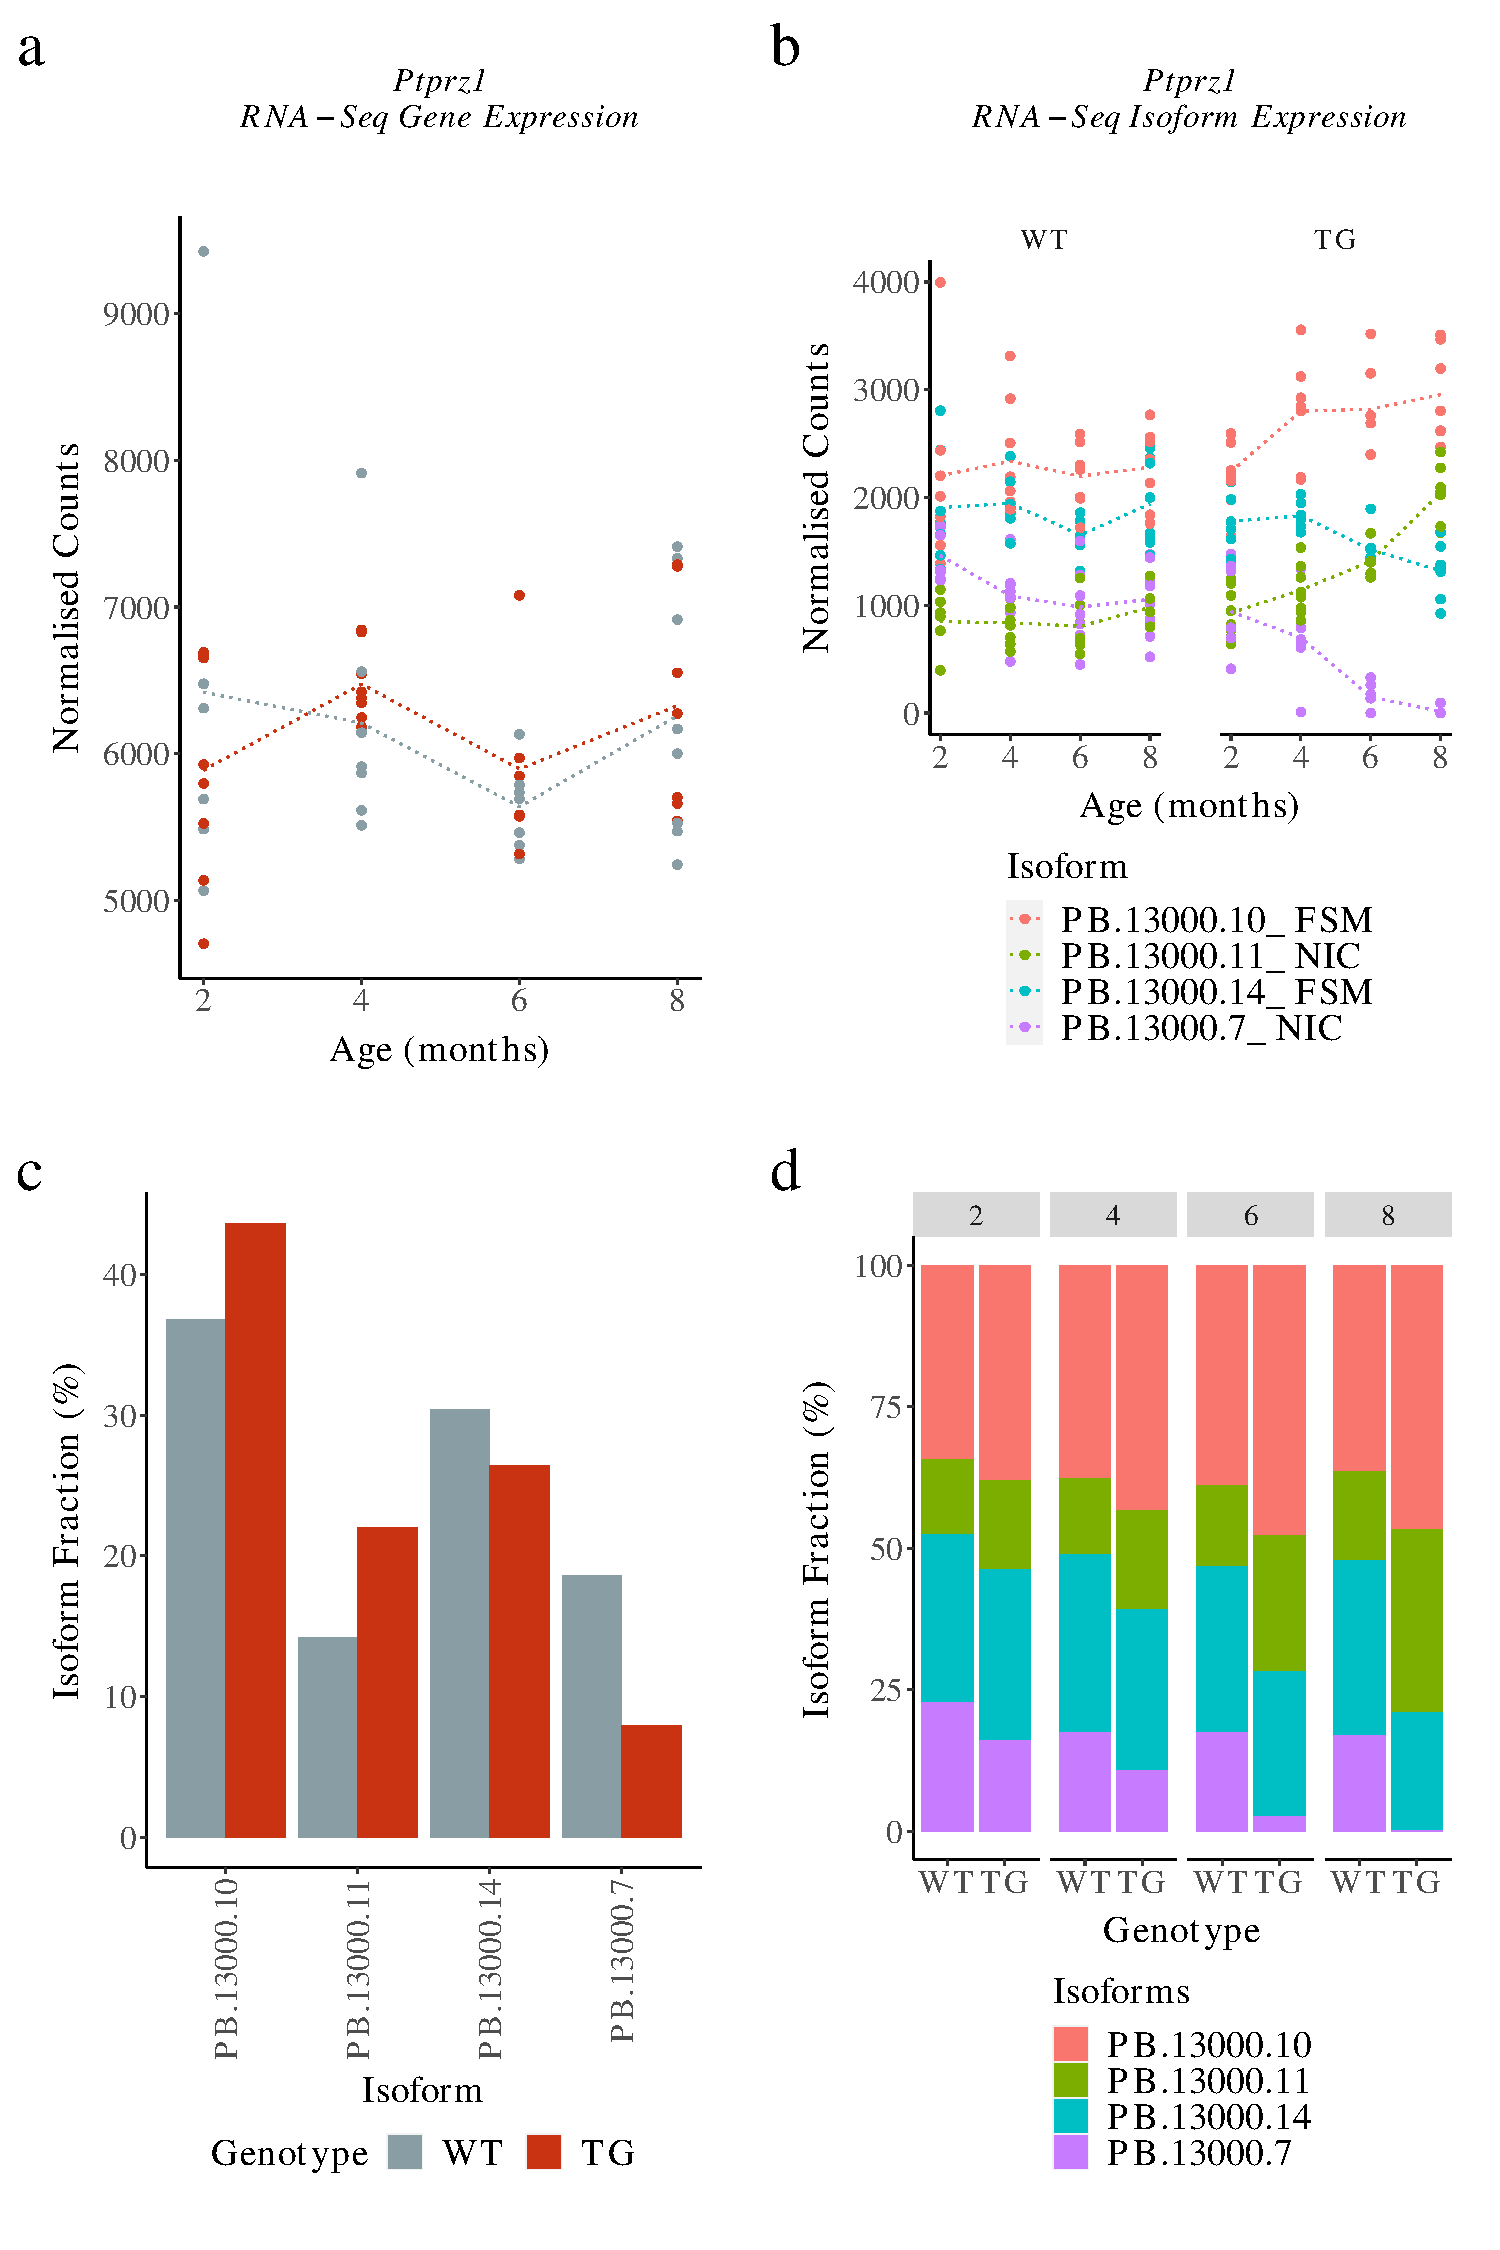
\includegraphics[page=1,scale = 0.55]{Figures/DIU_notDEG_nomajor.pdf}
	\end{center}
	\captionsetup{width=0.95\textwidth}
	\caption[Differential isoform expression and usage of \textit{Ptprz1}]%
	{\textbf{Differential isoform expression and usage of \textit{Ptprz1}}: \textbf{a)} \textit{Cisd3}'s RNA-Seq gene expression in wild-type (grey) and transgenic (red) mice, with no significant overall change. \textbf{b)} RNA-Seq expression of the two known and two novel isoforms in wild-type and mice across age. \textbf{c)} Overall isoform fraction of two isoforms across wild-type and transgenic, \textbf{d)} and by age.}    
	\label{fig:DIU_ptprz1}
\end{figure}


\begin{figure}[htp]
	\begin{center}
		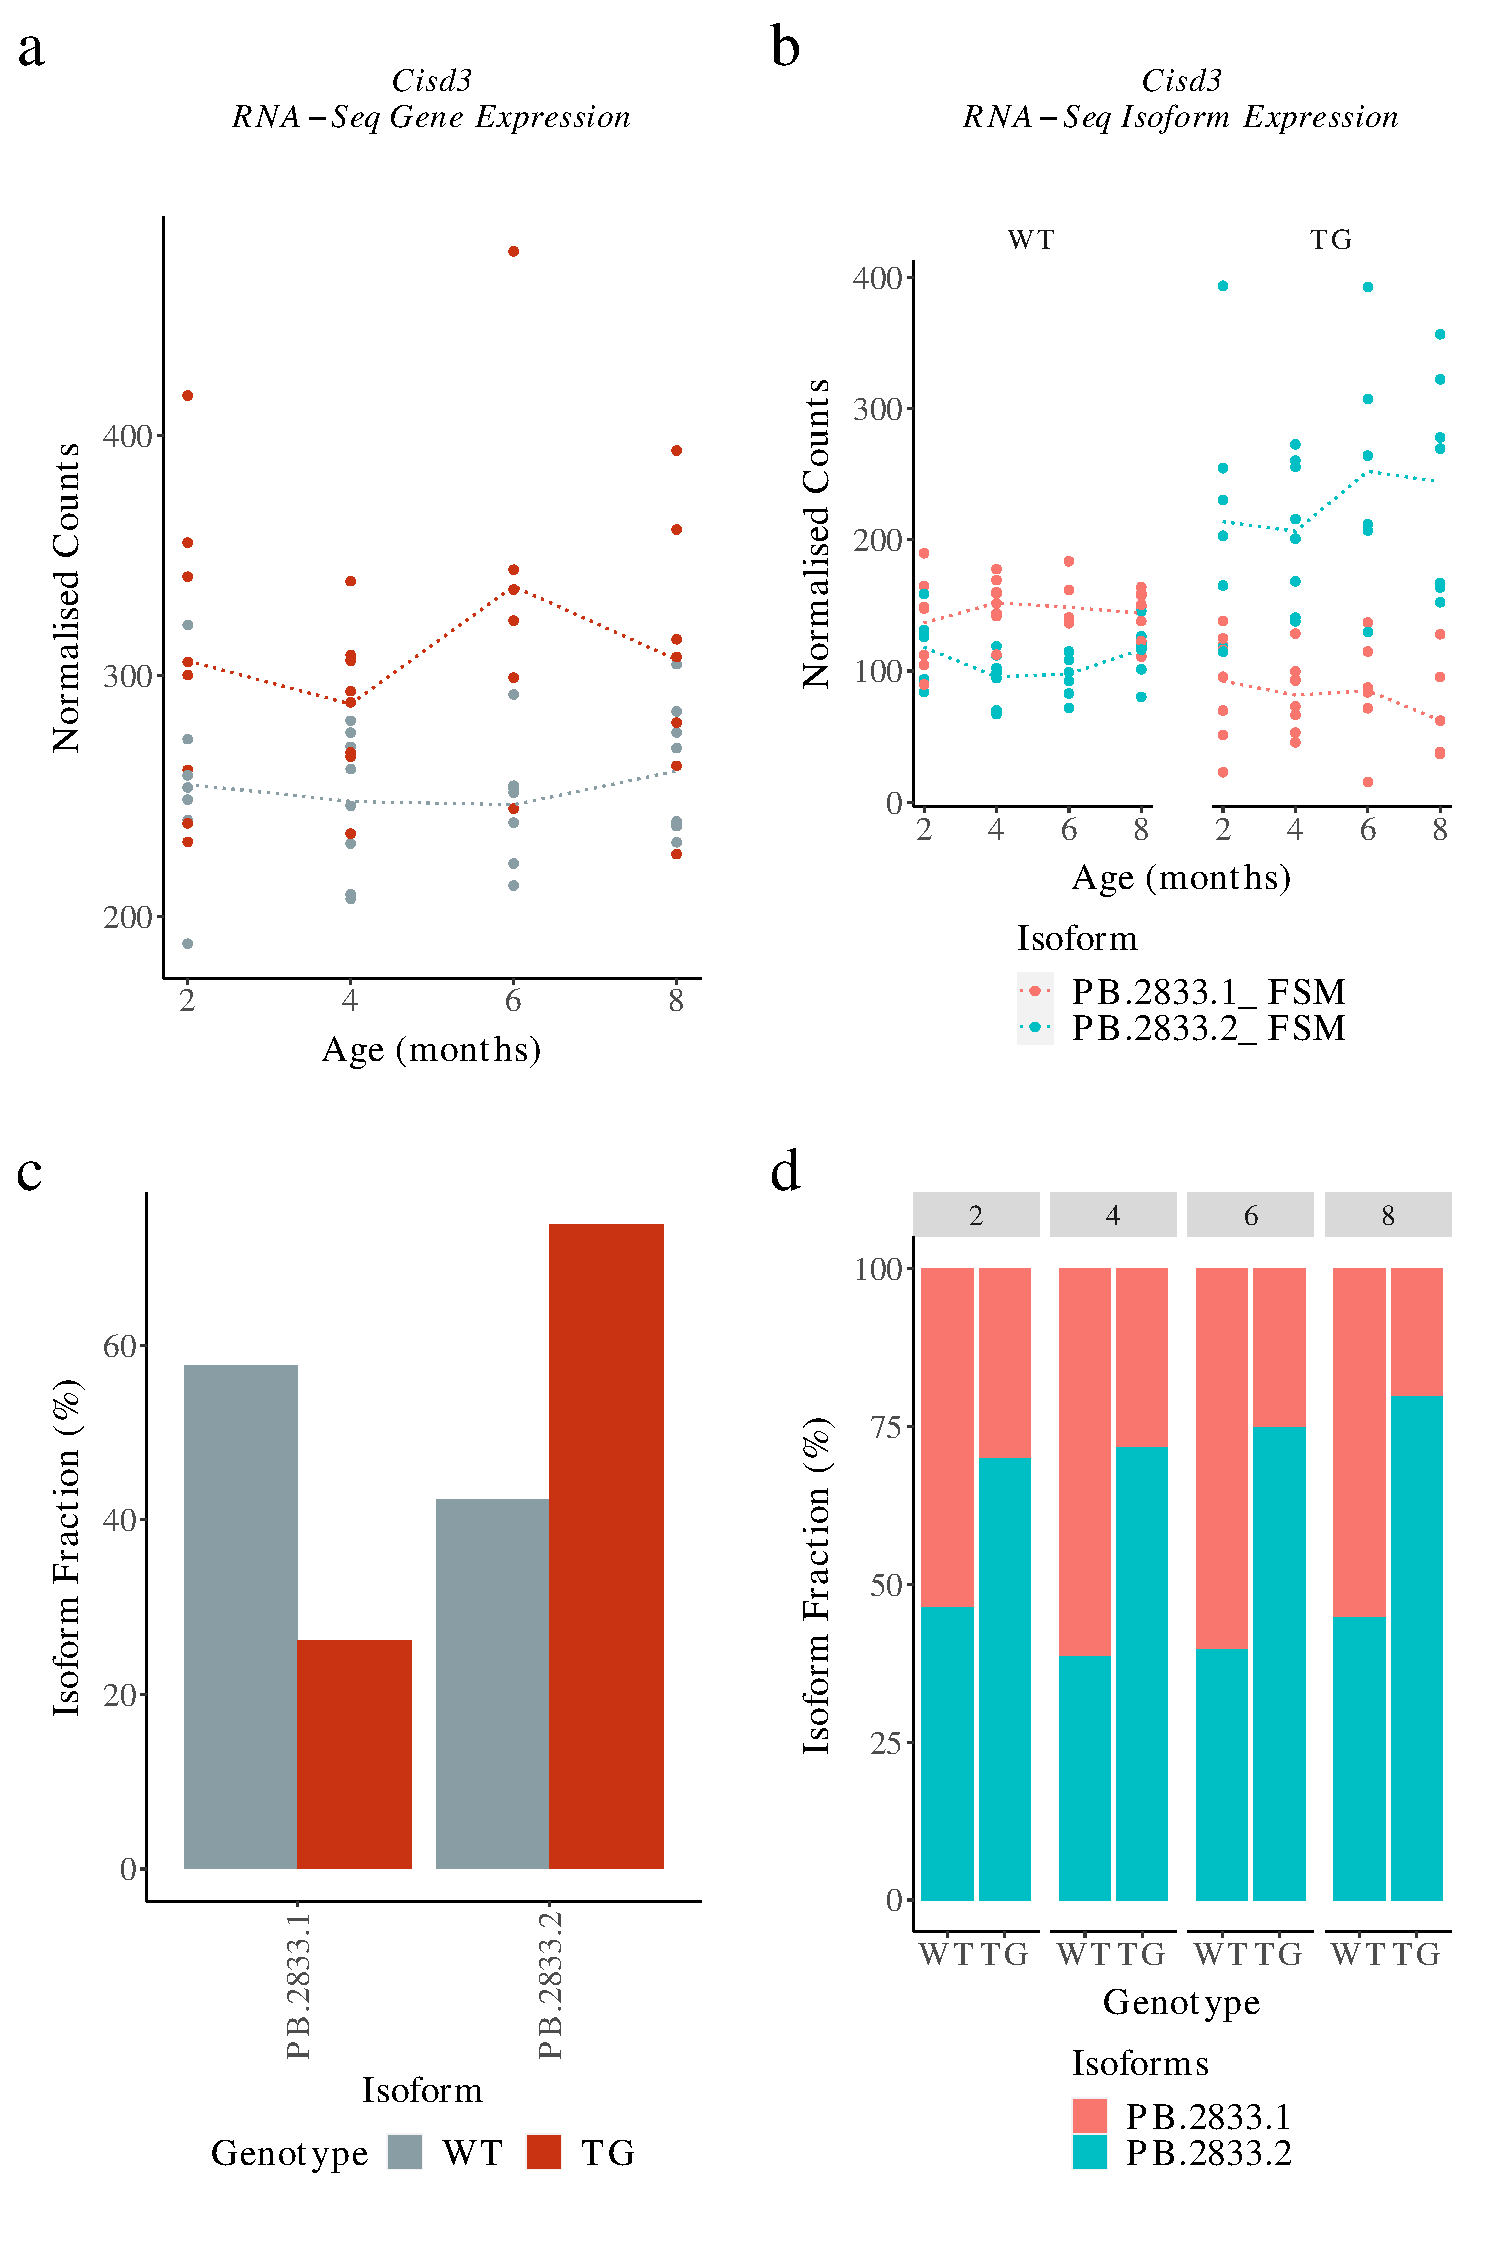
\includegraphics[page=1,scale = 0.55]{Figures/DIU_notDEG_major.pdf}
	\end{center}
	\captionsetup{width=0.95\textwidth}
	\caption[Differential isoform expression and usage of \textit{Cisd3}]%
	{\textbf{Differential isoform expression and usage of \textit{Cisd3}}: \textbf{a)} \textit{Cisd3}'s RNA-Seq gene expression in wild-type (grey) and transgenic (red) mice, with no significant overall change. \textbf{b)} RNA-Seq expression of the two known isoforms in wild-type and mice across age. \textbf{c)} Overall isoform fraction of two isoforms across wild-type and transgenic, \textbf{d)} and by age.}    
	\label{fig:DIU_Cisd3}
\end{figure}




\clearpage
\subsection{Differential Polyadenylation}

\clearpage
\subsection{Integration of splicing and methylation}
Epigenetic modifications such as DNA methylation have been widely acknowledged to heavily influence gene regulation and more specifically, alternative splicing. Using genome-wide DNA methylation data on the same mouse samples, we wanted to use an integrative approach to identify genes with both splicing and methylation changes between wild-type and transgenic mice. Genes defined to undergo differential splicing were classified by either genes with a change in transcript expression (differential isoform expression - DIE), a change in usage of isoform proportions (differential isoform usage - DIU) or a change in feature element (differential feature inclusion - DFI). Genes with changes in methylation were classified as either with a change in a specific position (differential methylated position - DMP) associated with tau pathology (genotype effect) and progressively over time (interaction effect), or associated with a cluster of differentially methylated cytosines (differentially methylated region - DMR). 

Using a stringent approach to identify biologically meaningful splicing changes, we identified nine genes with an altered splicing and methylation profile associated with progressive tau pathology. The most significant co-differentially-methylated position and differentially-spliced gene was \textit{Spata13} - a gene involved in cell migration\cite{Bourbia2019} and has been reported to be upregulated in entorhinal cortex of AD patients\cite{Yan2019} - which was characterised with a change in transcript expression, usage and feature inclusion. There was a significant progressive increase in expression of the shorter known isoform (PB.4966.2, ENSMUST00000162945.1) in the transgenic mice, whereas there was no change in expression of the longer, novel NIC isoform (PB.4966.1) which harboured a 5' miRNA-binding site (miR-446h-5p) and an alternative transcription start site with an upstream open reading frame. A DMP was identified upstream of \textit{Spata13} (8.9Kb and 107Kb from known and novel isoform respectively) and was hypermethylated in transgenic mice compared to wild-type, suggesting a distal suppressed expression of both isoforms in the wild-type. Conversely, the decreased methylation in the transgenic is only associated with suppressed expression of the proximal, novel isoform. 

%Another gene with co-differentially-methylated position and differentially-spliced gene was \textit{Tmem237}, characterised by an isoform switch of a known (PB.261.4) and novel NNC (PB.261.10) isoform, which had an alternative first exon and a shorter 3'UTR resulting in absence of miRNA-binding sites. 
% check methylation levels across first exon.

Other genes were characterised with a change in transcript expression correlated with a change in methylation. This included \textit{Ncf2}, \textit{Osmr}, and \textit{Cebpa} where there was a progressive increase in expression of the respective known isoform and an associated hypomethylated DMP (located in the promoter) in transgenic; whereas in \textit{Rnf165} and \textit{Susd5}, there was a progressive downregulation of known isoform and an associated hypermethylated DMP in transgenic. Interestingly, we also identified altered splicing and methylation changes in \textit{Irf8} - a transcription factor of the IRF family that is involved in microglial activation in AD\cite{Zeng2017}, where a hypomethylated DMP (located upstream) in TG was associated with progressive increase in transcript expression. The associations described here between DNA methylation and transcript expression support well-established theories of the relationship between DNA methylation and gene expression, whereby increased methylation at the promoter is associated with decreased gene expression. Of note, only one isoform was detected for each of these genes.  
% Note other example where this was not the case 

Focusing on genotype-associated differentially methylated regions, we identified splicing changes annotated to \textit{As3mt} and \textit{Prnp}. Three isoforms were detected for \textit{As3mt}, a schizophrenia-associated GWAS gene, whereby there was a progressive upregulation in the known isoform (PB.8363.2, ENSMUST00000003655.8) in TG (P = 4.98 x 10\textsuperscript{-18}, R\textsuperscript{2} = 0.56) while there was no detected change in expression of the two other novel NNC isoforms, both of which were characterised by a novel splice junction resulting in a novel exon that was absent in the known isoform. A DMR consisting of X differentially methylated cytosine was identified XX upstream of this novel exon within the intron, and was hypermethylated in transgenic mice compared to wild-type ($\Delta$ = 0.19, P = 1.22 x 10\textsuperscript{-8}). We hypothesise that an increase in methylation in this region would hinder recruitment and assembly of the spliceosome, resulting in skipping of the novel exon and subsequent increased expression of the known isoform. 

There was an increase in expression of a novel isoform of \textit{Prnp} in transgenic mice. However, given that \textit{Mapt} transgene includes exons 2 and 3 of the \textit{Prnp}, we were uncertain whether the transcript expression changes attributed to \textit{Prnp} from short-read RNA-Seq reads was due to the mouse gene or the human transgene. No change in transcript expression was identified from Iso-Seq full-length read counts. 
